%%%%%%%%%%%%%%%%%%%%%%%%%%%%%%%%%%%%%%%%%
% Beamer Presentation
% LaTeX Template
% Version 1.0 (10/11/12)
%
% This template has been downloaded from:
% http://www.LaTeXTemplates.com
%
% License:
% CC BY-NC-SA 3.0 (http://creativecommons.org/licenses/by-nc-sa/3.0/)
%
%%%%%%%%%%%%%%%%%%%%%%%%%%%%%%%%%%%%%%%%%

%----------------------------------------------------------------------------------------
%	PACKAGES AND THEMES
%----------------------------------------------------------------------------------------

\documentclass{beamer}

\mode<presentation> {

% The Beamer class comes with a number of default slide themes
% which change the colors and layouts of slides. Below this is a list
% of all the themes, uncomment each in turn to see what they look like.

%\usetheme{default}
%\usetheme{AnnArbor}
%\usetheme{Antibes}
%\usetheme{Bergen}
%\usetheme{Berkeley}
%\usetheme{Berlin}
%\usetheme{Boadilla}
%\usetheme{CambridgeUS}
%\usetheme{Copenhagen}
%\usetheme{Darmstadt}
%\usetheme{Dresden}
%\usetheme{Frankfurt}
%\usetheme{Goettingen}
%\usetheme{Hannover}
%\usetheme{Ilmenau}
%\usetheme{JuanLesPins}
%\usetheme{Luebeck}
\usetheme{Madrid}
%\usetheme{Malmoe}
%\usetheme{Marburg}
%\usetheme{Montpellier}
%\usetheme{PaloAlto}
%\usetheme{Pittsburgh}
%\usetheme{Rochester}
%\usetheme{Singapore}
%\usetheme{Szeged}
%\usetheme{Warsaw}

% As well as themes, the Beamer class has a number of color themes
% for any slide theme. Uncomment each of these in turn to see how it
% changes the colors of your current slide theme.

%\usecolortheme{albatross}
%\usecolortheme{beaver}
%\usecolortheme{beetle}
%\usecolortheme{crane}
%\usecolortheme{dolphin}
%\usecolortheme{dove}
%\usecolortheme{fly}
%\usecolortheme{lily}
%\usecolortheme{orchid}
%\usecolortheme{rose}
%\usecolortheme{seagull}
%\usecolortheme{seahorse}
%\usecolortheme{whale}
%\usecolortheme{wolverine}

%\setbeamertemplate{footline} % To remove the footer line in all slides uncomment this line
%\setbeamertemplate{footline}[page number] % To replace the footer line in all slides with a simple slide count uncomment this line

%\setbeamertemplate{navigation symbols}{} % To remove the navigation symbols from the bottom of all slides uncomment this line
}

\usepackage{graphicx} 
\usepackage{booktabs} 
\usepackage{hyperref}
\usepackage{tikz}
\usepackage{amsmath}
\usepackage{epstopdf}

%----------------------------------------------------------------------------------------
%	TITLE PAGE
%----------------------------------------------------------------------------------------

\title[Introduction]{Systems and control theory}

\author{} % Your name
\institute[KU Leuven] % Your institution
{
Katholieke Universiteit Leuven \\ % Your institution
\medskip
\textit{} % Your email address
}
\date{\today}

\begin{document}

\begin{frame}
\titlepage
\end{frame}

\begin{frame}
\frametitle{Overview} 
\tableofcontents
\end{frame}

%----------------------------------------------------------------------------------------
%	PRESENTATION SLIDES
%----------------------------------------------------------------------------------------

%------------------------------------------------
\section{Course overview} 
%------------------------------------------------

\begin{frame}
\frametitle{Course overview}
\begin{enumerate}
\item Introduction
\item Classification of systems
\item System modelling
\item Discrete time systems
\item Continuous time systems
\item Frequency response of dynamical systems
\item Discretizations of continuous time systems
\item Introduction to control
\item Design in the frequency domain and Nyquist stability criterion
\item Lead and lag compensators
\item PID control
\end{enumerate}
\end{frame}

%------------------------------------------------

%\begin{frame}
%\frametitle{Learning objectives}
%- Analyse of iscrete time and continuous systems with different methods\\
%- Design of controller that has to satisfy certain requirements
%\end{frame}

%------------------------------------------------

\begin{frame}
\frametitle{Methodology and evaluation}
\begin{itemize}
\item 20 lectures \\
\item 8 excercise sessions\\
\item Learning platform: Sofia\\
\url{www.sofialearn.com}\\
Course: Systems and control theory\\
Material from the lectures (powerpoints, video's), assignments for exercise sessions and supplementary material (downloads, tutorials, books, links, journals, conferences)\\
\bigskip
\textbf{Exam}
\item Written exam
\item You can bring: course book, calculator
\item Duration: 4h
\end{itemize}
\end{frame}

%------------------------------------------------

\begin{frame}
\frametitle{}
\center{\textbf{\huge{Introduction}}}
\end{frame}

%------------------------------------------------
\section{Systems theory} 
%------------------------------------------------

\begin{frame}
\frametitle{Systems theory}
System theory occupies itself with the mathematical description and study of systems.
Models describe the connections between input and output.\\
\bigskip
\begin{figure}
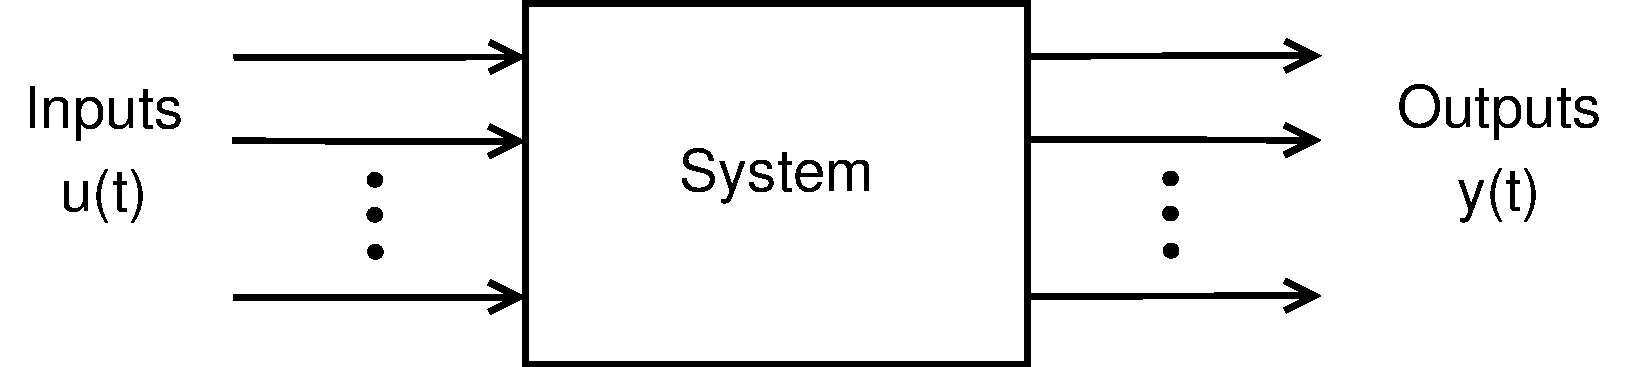
\includegraphics[width=.8\linewidth]{systems_theory}
\end{figure}
Next to inputs and outputs, states (denoted by \textbf x) are a third type of variable used to describe a system. They represent the internal state of the system at a given time. The next state is a function of the previous states.
The order of a system is the number of state-variables (i.e. the size of the vector \textbf x).\\
\bigskip
%Dynamical systems can be devided into two types: \textbf{discrete} and \textbf{continuous} systems.
\end{frame}

%------------------------------------------------
%\subsection{Discrete systems} 
%
%
%\begin{frame}
%\frametitle{Discrete systems}
%
%\begin{columns}[c]
%
%\column{.3\textwidth}
%\centering \textbf{Delay element}\\
%\bigskip
%\begin{tikzpicture}
%\draw (2,1) rectangle (3,2) node[pos=.5] {D}; 
%\end{tikzpicture}
%
%\column{.3\textwidth}
%\centering \textbf{Adder}\\
%\bigskip
%\begin{tikzpicture}
%\draw (0,-.8) circle (.5cm) node (0,-.8) {+}; 
%\end{tikzpicture}
%
%\column{.3\textwidth}
%\centering \textbf{Constant multiplier}\\
%\bigskip
%\begin{tikzpicture}
%\draw (0,-.8) circle (.5cm) node (0,-.8) {a}; 
%\end{tikzpicture}
%
%\end{columns}
%
%\bigskip
%Restrictions:
%\begin{columns}[c]
%
%\column{.5\textwidth}
%\begin{figure}
%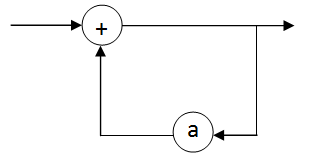
\includegraphics[width=.85\linewidth]{loop}
%\end{figure}
%No loops without delay element
%
%\column{.5\textwidth}
%\begin{figure}
%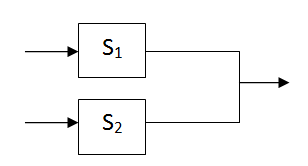
\includegraphics[width=.8\linewidth]{connected_output}
%\end{figure}
%No connecting outputs without adder
%
%\end{columns}
%
%\end{frame}
%
%%------------------------------------------------
%
%\begin{frame}
%\frametitle{Example}
%\begin{figure}
%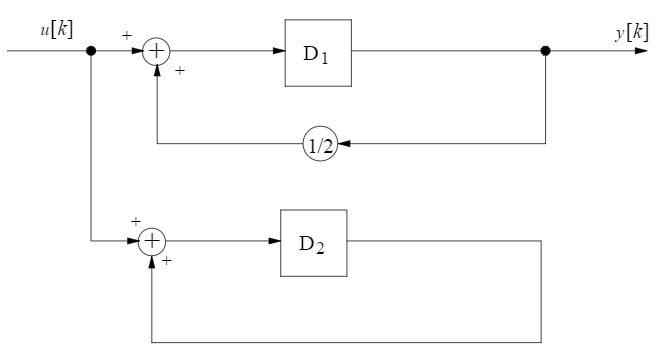
\includegraphics[width=1\linewidth]{discrete_system}
%\end{figure}
%
%\end{frame}
%
%%------------------------------------------------
%
%\begin{frame}
%\frametitle{Methods}
%\textbf{State space representation}\\
%$x[k+1] \> = A\; x[k] + B\; u[k]$ \\
%$y[k]\qquad = C\; x[k] + C\; u[k]$
%\bigskip
%
%\textbf{Difference equations}\\
%$\sum\limits_{i=0}^n a_{i}y[k+i] = \sum \limits_{i=0}^n b_{i}u[k+i]$
%\bigskip
%
%\textbf{Impulse response}\\
%$h[k] = y[k] \> when \> u[k] = \delta[k]$\\
%\bigskip
%
%\textbf{Z-transform}\\
%$X(z) = \sum \limits_{k = -\infty}^{+\infty} x[k] z^{-k}$
%\bigskip
%
%\textbf{Transfer function}\\
%$H(z) = \frac{Y(z)}{U(z)} \; \Rightarrow \> Y(z) = H(z)U(z)$
%
%\end{frame}
%
%%------------------------------------------------
%\subsection{Continuous systems} 
%
%\begin{frame}
%\frametitle{Continuous systems}
%
%\begin{columns}[c]
%
%\column{.3\textwidth}
%\centering \textbf{Integrator}\\
%\bigskip
%\begin{tikzpicture}
%\draw (2,1) rectangle (3,2) node[pos=.5] {$\int$}; 
%\end{tikzpicture}
%
%\column{.3\textwidth}
%\centering \textbf{Adder}\\
%\bigskip
%\begin{tikzpicture}
%\draw (0,-.8) circle (.5cm) node (0,-.8) {+}; 
%\end{tikzpicture}
%
%\column{.3\textwidth}
%\centering \textbf{Constant multiplier}\\
%\bigskip
%\begin{tikzpicture}
%\draw (0,-.8) circle (.5cm) node (0,-.8) {a}; 
%\end{tikzpicture}
%
%\end{columns}
%
%\bigskip
%Restrictions:
%\begin{columns}[c]
%
%\column{.5\textwidth}
%\begin{figure}
%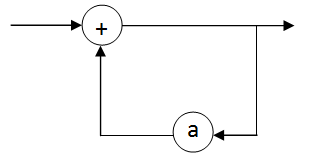
\includegraphics[width=.85\linewidth]{loop}
%\end{figure}
%No loops without integrator
%
%\column{.5\textwidth}
%\begin{figure}
%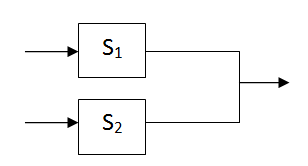
\includegraphics[width=.8\linewidth]{connected_output}
%\end{figure}
%No connecting outputs without adder
%
%\end{columns}
%
%\end{frame}
%
%%------------------------------------------------
%
%\begin{frame}
%\frametitle{Example}
%\begin{figure}
%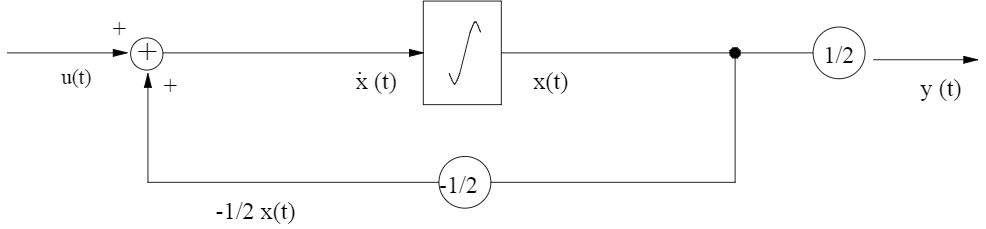
\includegraphics[width=1\linewidth]{continuous_system}
%\end{figure}
%
%\end{frame}
%%------------------------------------------------
%
%\begin{frame}
%\frametitle{Methods}
%\textbf{State space representation}\\
%$\dot{x}(t) \> = A \;x(t) + B\; u(t)$ \\
%$y(t)\> = C\; x(t) + C\; u(t)$
%\bigskip
%
%\textbf{Differential equations}\\
%$\sum\limits_{i=0}^n a_{i}y^{(i)} = \sum \limits_{i=0}^n b_{i}u^{(i)}$
%\bigskip
%
%\textbf{Impulse response}\\
%$h(t) = y(t) \> when \> u(t) = \delta(t)$\\
%\bigskip
%
%\textbf{Laplace transform}\\
%$X(s) = \int_0^\infty \! e^{-st}f(t) \, \mathrm{d}t$
%\bigskip
%
%\textbf{Transfer function}\\
%$H(s) = \frac{Y(s)}{U(s)} \; \Rightarrow \> Y(s) = H(s)U(s)$
%
%\end{frame}



%------------------------------------------------
\section{Dynamical systems} 
%------------------------------------------------

\begin{frame}
\frametitle{Dynamical system}
A dynamical system is a constantly changing system that connects outputs (denoted by \textbf y) and inputs (denoted by \textbf u).\\The word dynamical refers to the fact that its current output depends on past input, contrary to static systems where the current output only depends on current input. This means that in a dynamical system the output changes with time if the system is not in a state of equilibrium.
\begin{figure}
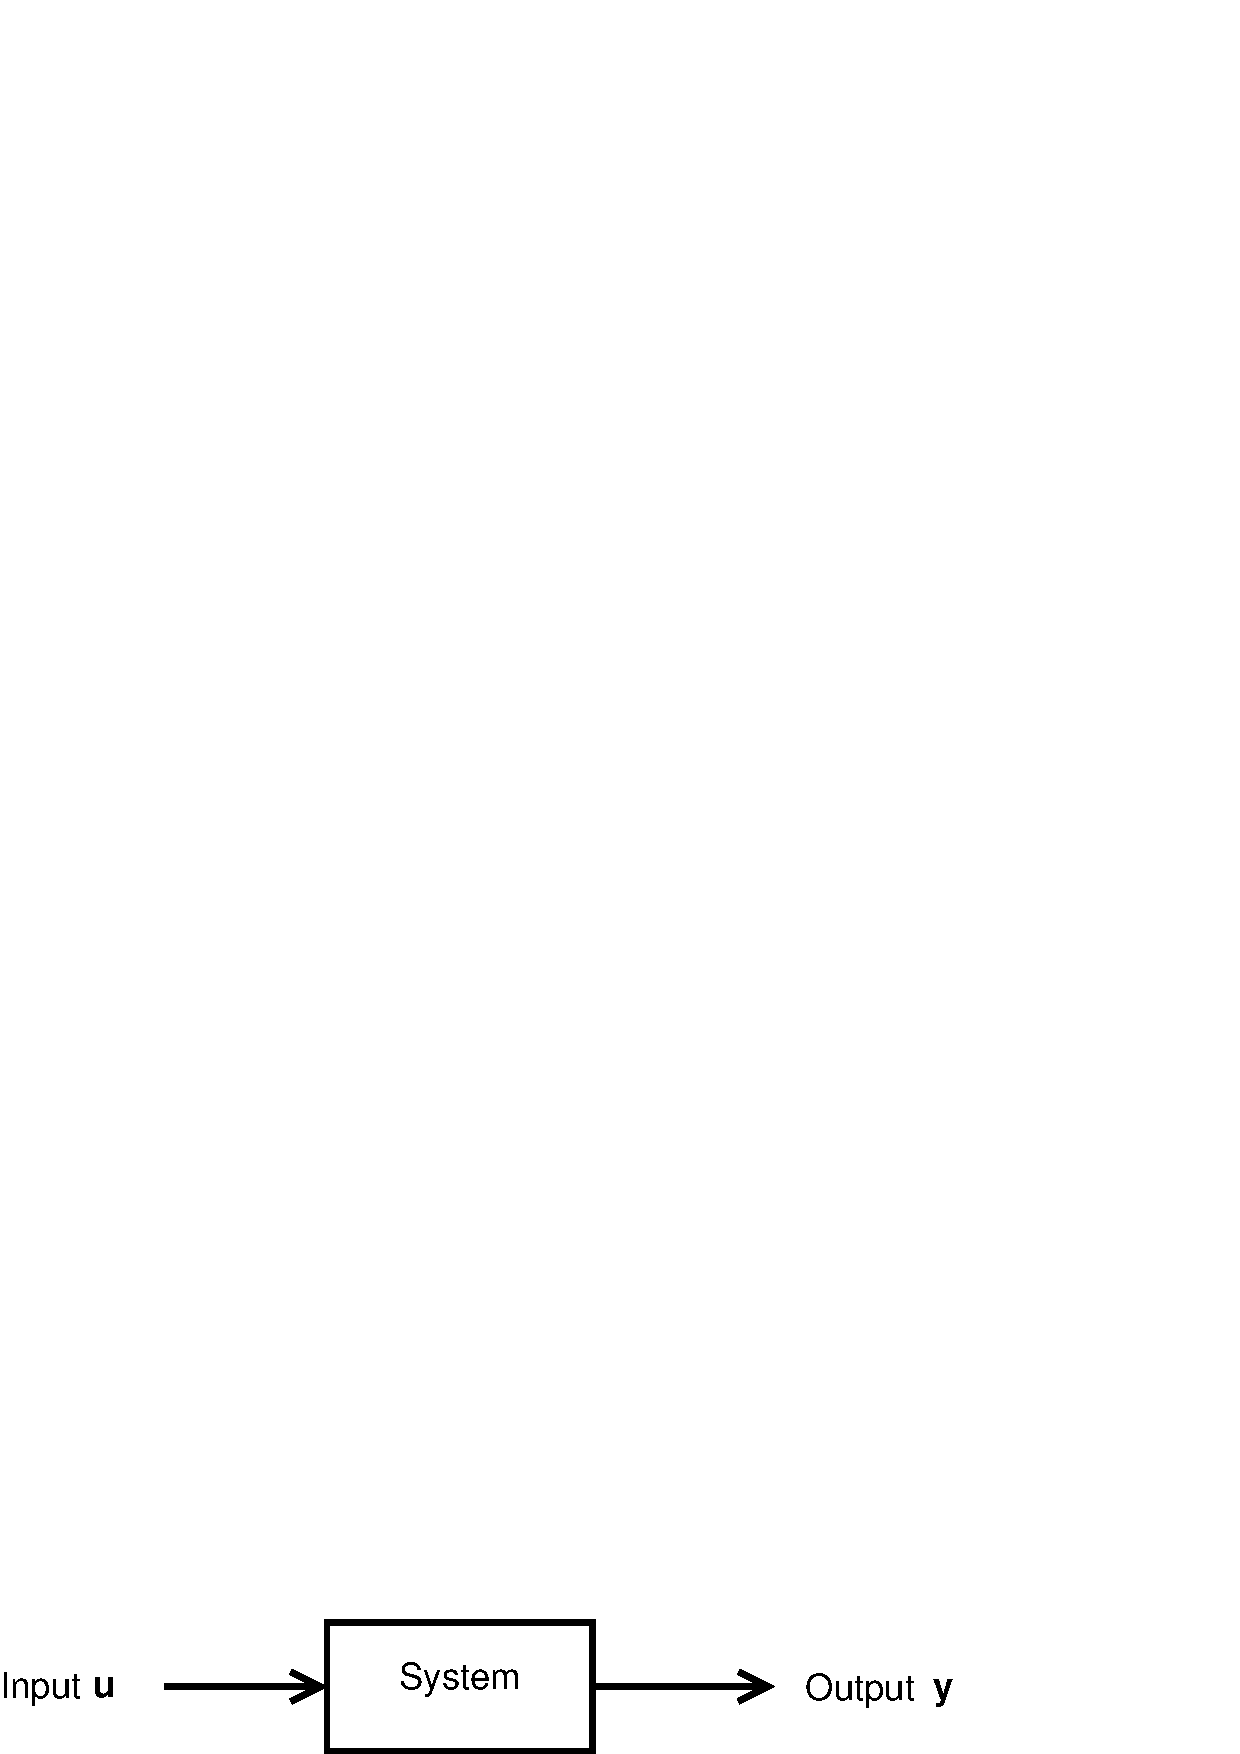
\includegraphics[width=0.8\linewidth]{Dynamical_system}
\end{figure}
\medskip
Everything is a dynamical system.
\end{frame}

%------------------------------------------------
\section{Real life examples} 
%------------------------------------------------

\begin{frame}
\frametitle{Millenium Bridge}
Resonance on the Millenium Bridge in London due to the rithm of walking people.
\begin{figure}
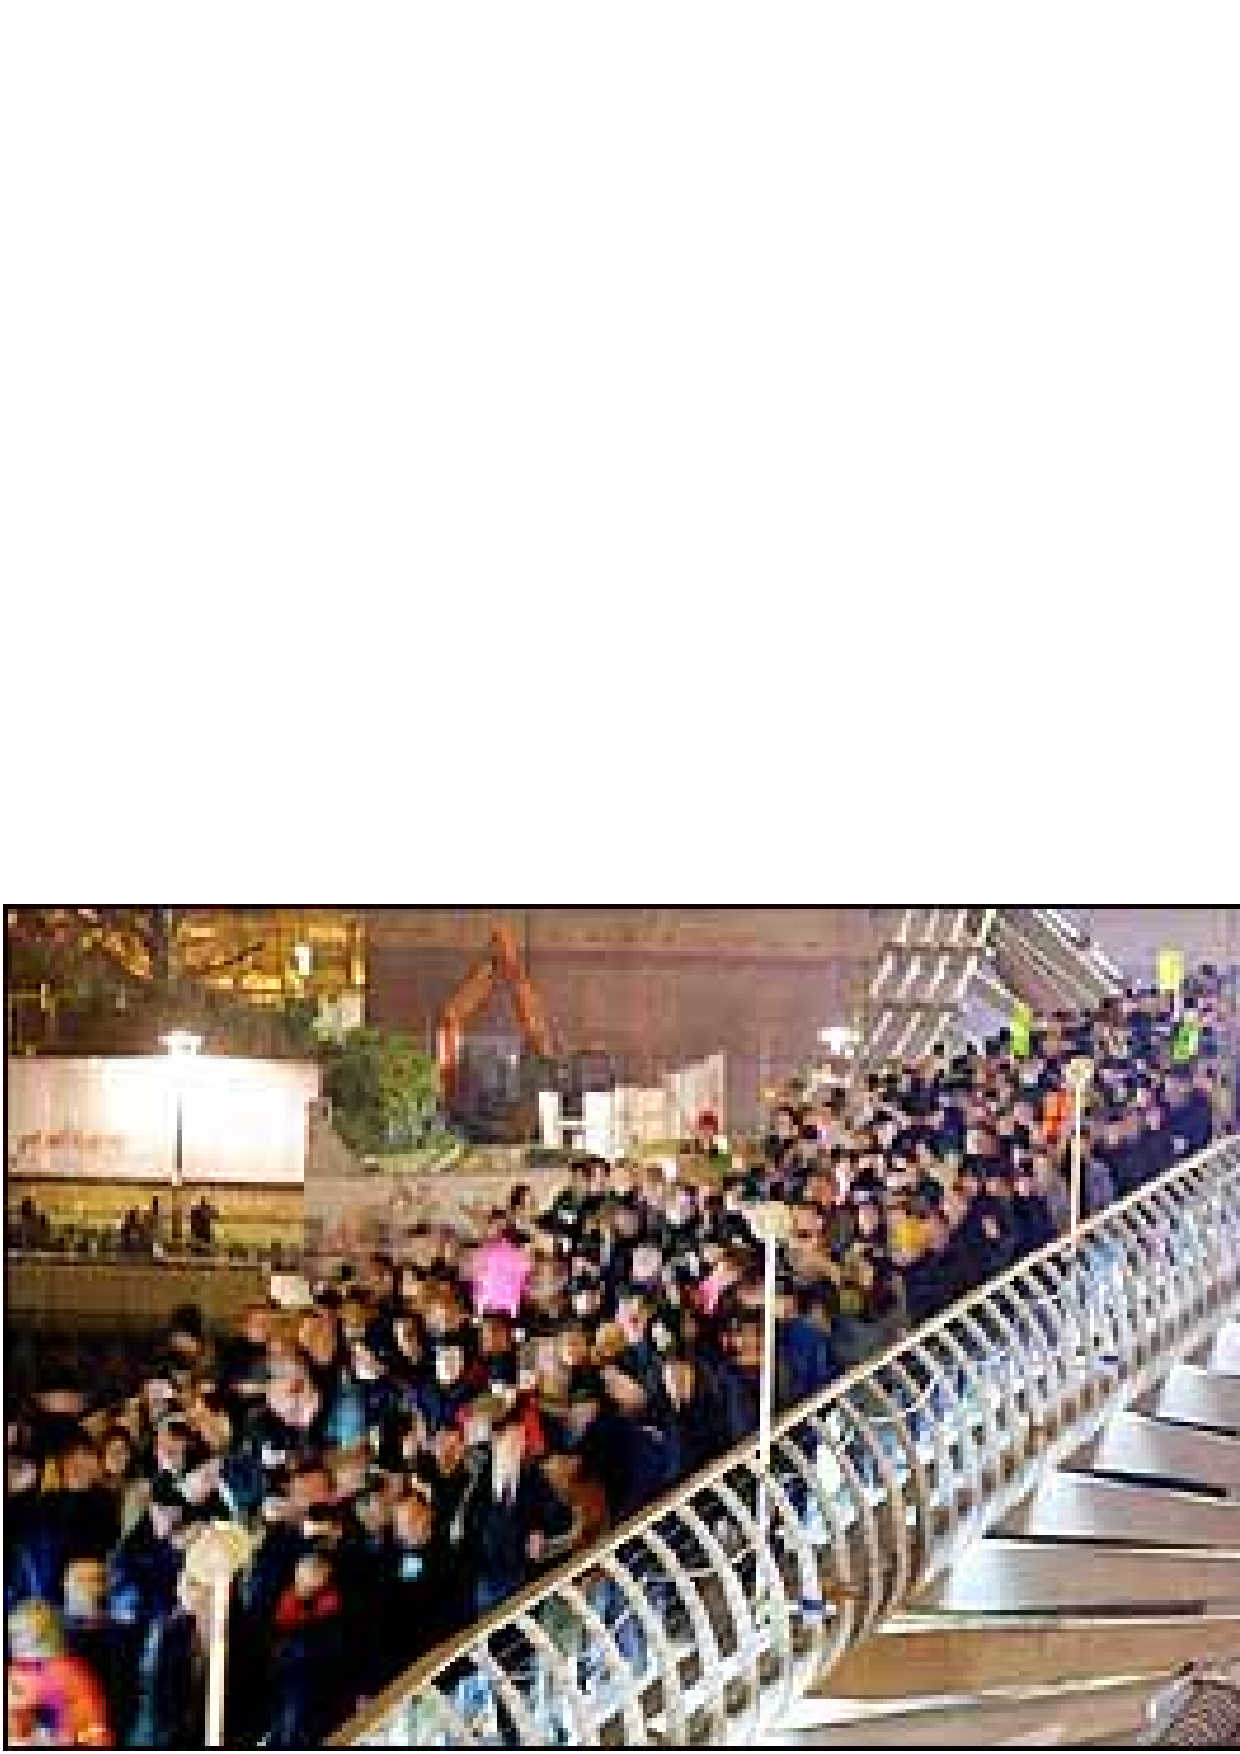
\includegraphics[scale=0.4]{millenium_bridge}
\end{figure}
\url{https://www.youtube.com/watch?v=eAXVa__XWZ8}
\end{frame}

%------------------------------------------------

\begin{frame}
\frametitle{Neuronal acitvity}
Real-time visualization of neuronal activity in the zebrafish brain
\begin{figure}
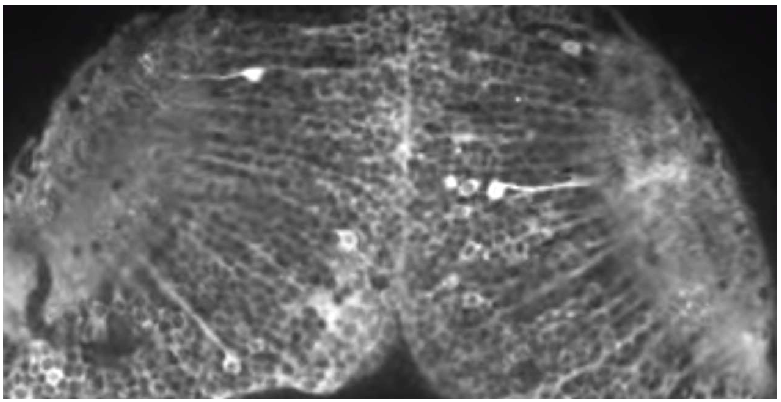
\includegraphics[scale=0.8]{neuronal_activity}
\end{figure}
\url{https://youtu.be/_rGEkYfQVwY}
\end{frame}

%------------------------------------------------

\begin{frame}
\frametitle{Drumstick hitting a cymbal}
Drumstick hitting a cymbal at 1000 frames/sec
\begin{figure}
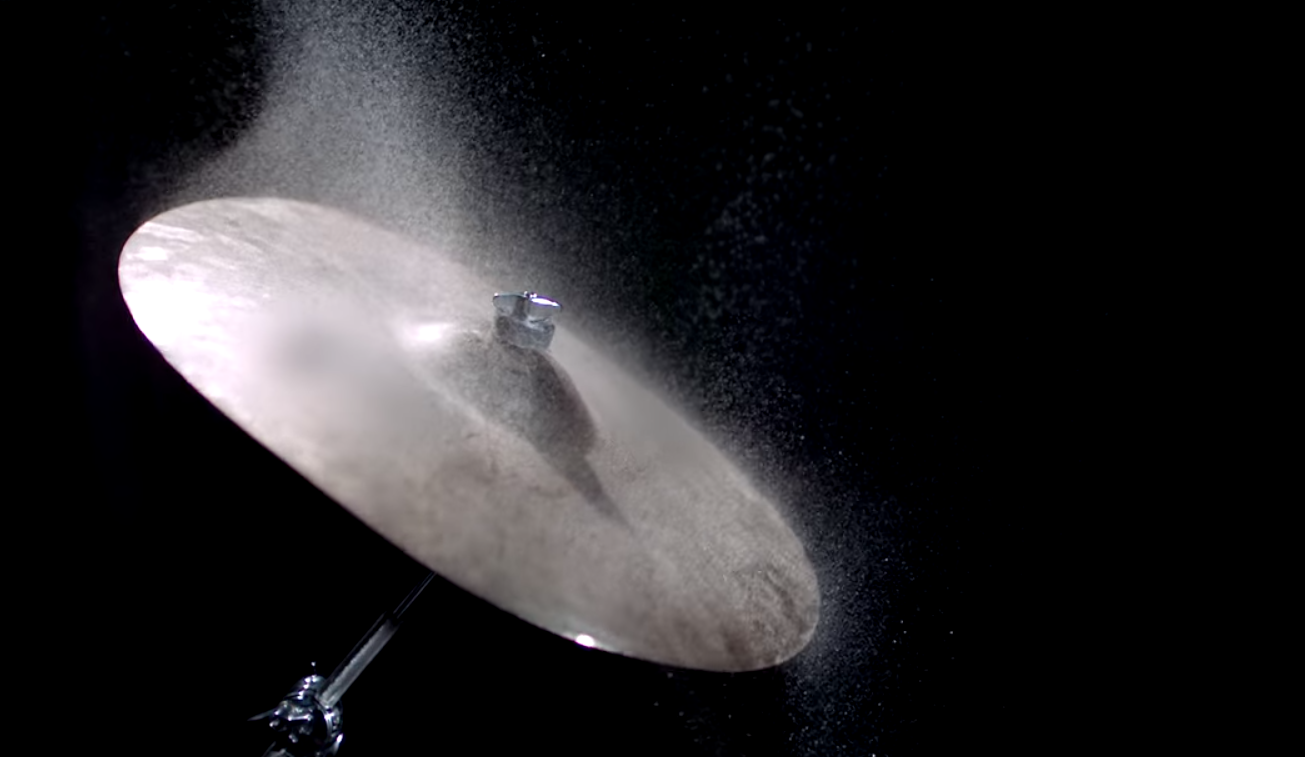
\includegraphics[scale=.8]{cymbal}
\end{figure}
\url{https://youtu.be/kpoanOlb3-w}
\end{frame}

%------------------------------------------------

\begin{frame}
\frametitle{Pilot making a risky maneuvre}
Experienced pilot making a risky maneuvre
\begin{figure}
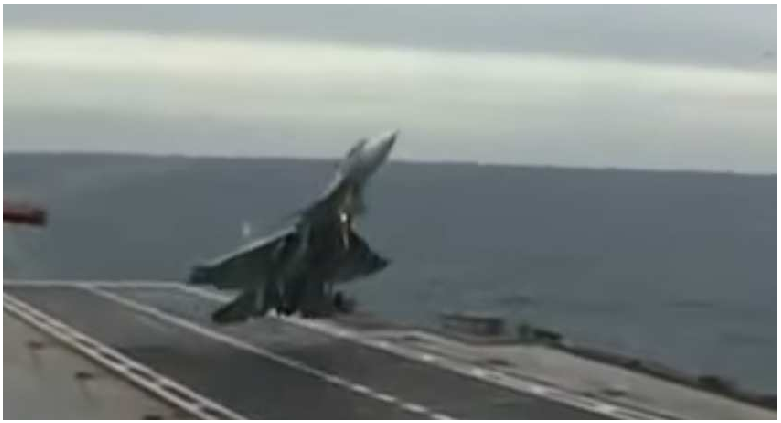
\includegraphics[scale=0.8]{risky_maneuvre}
\end{figure}
\url{https://youtu.be/gGnyWgXnZ6g}
\end{frame}

%------------------------------------------------

\begin{frame}
\frametitle{Synchronized metronomes}
Synchronized metronomes
\begin{figure}
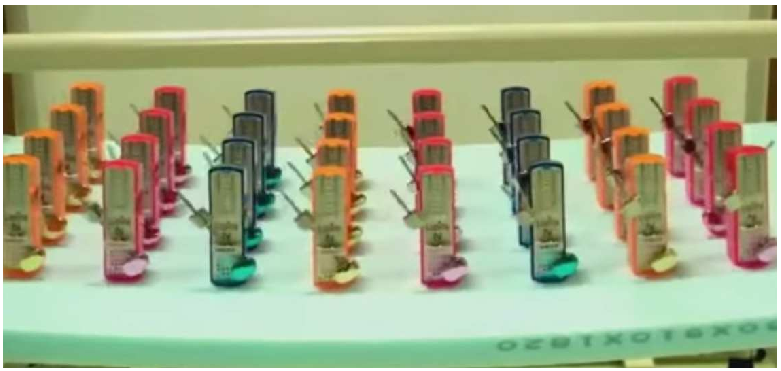
\includegraphics[scale=0.8]{synchronized_metronomes}
\end{figure}
\url{https://www.youtube.com/watch?v=5v5eBf2KwF8}
\end{frame}

%------------------------------------------------

%\begin{frame}
%\frametitle{Everything is a dynamical system}
%\textbf{Antique racecar}
%\begin{figure}
%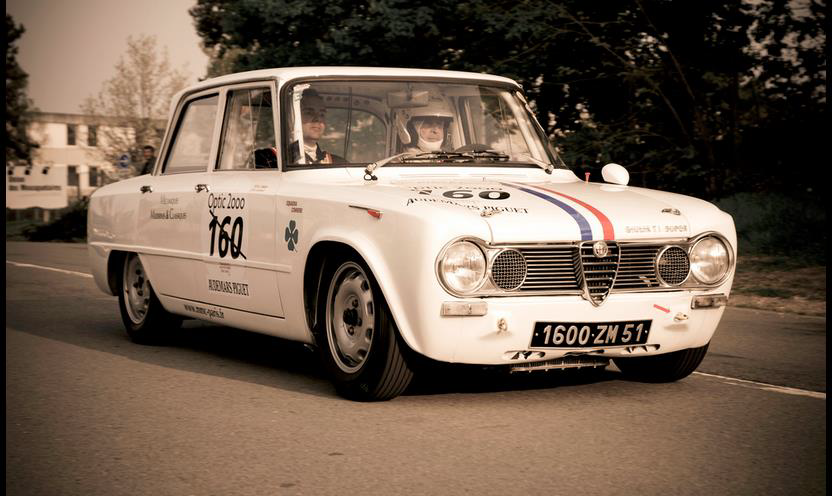
\includegraphics[width=0.9\linewidth]{racecar}
%\end{figure}
%\end{frame}
%
%%------------------------------------------------
%
%\begin{frame}
%\frametitle{Everything is a dynamical system}
%\textbf{Predator-prey system}
%\begin{figure}
%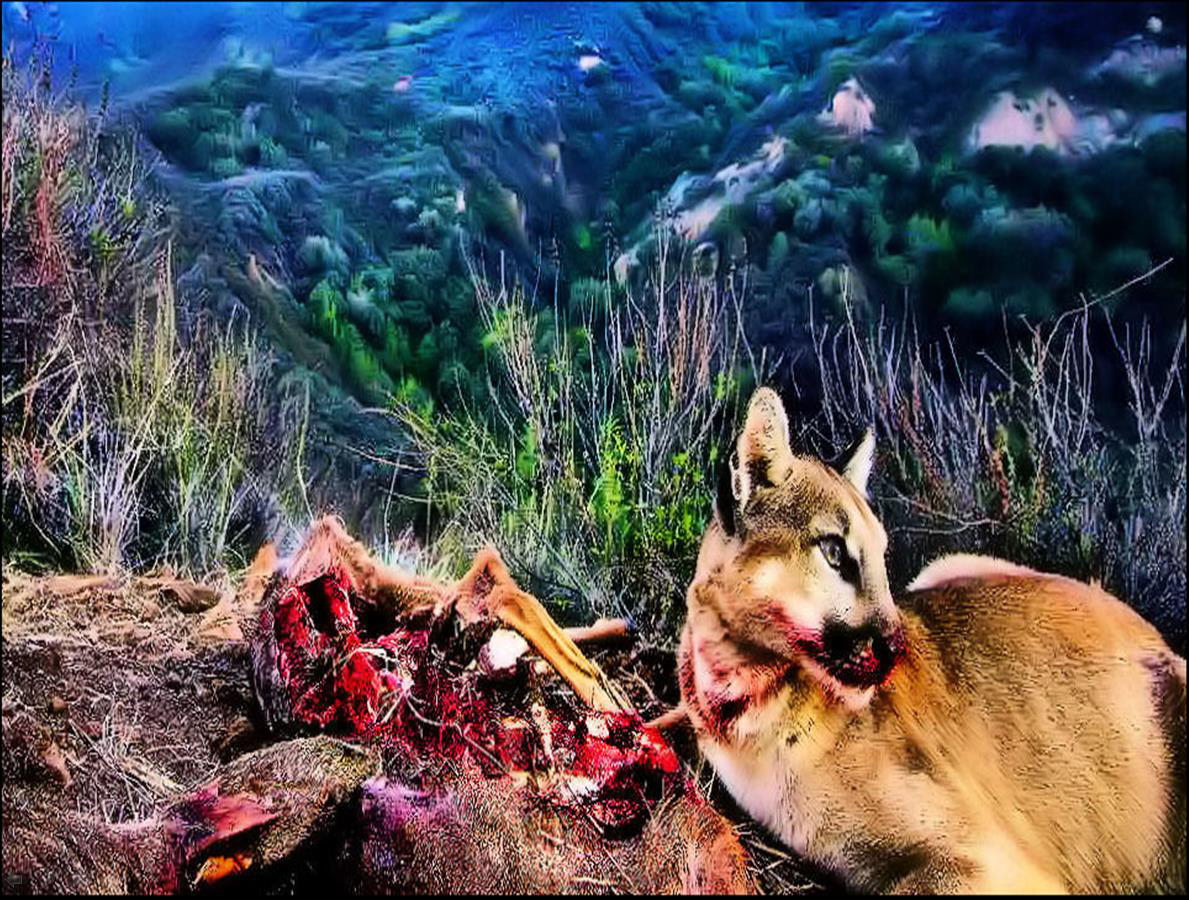
\includegraphics[width=0.8\linewidth]{predator_prey}
%\end{figure}
%\end{frame}

%------------------------------------------------
\section{Control theory}
%------------------------------------------------

\begin{frame}
\frametitle{Control theory}
Control theory deals with the behavior of dynamical systems and how their behavior is modified by feedback.\\
The output is compared to the reference input and this \textit{'error'} is used to adjust the system. 
\bigskip
\begin{figure}
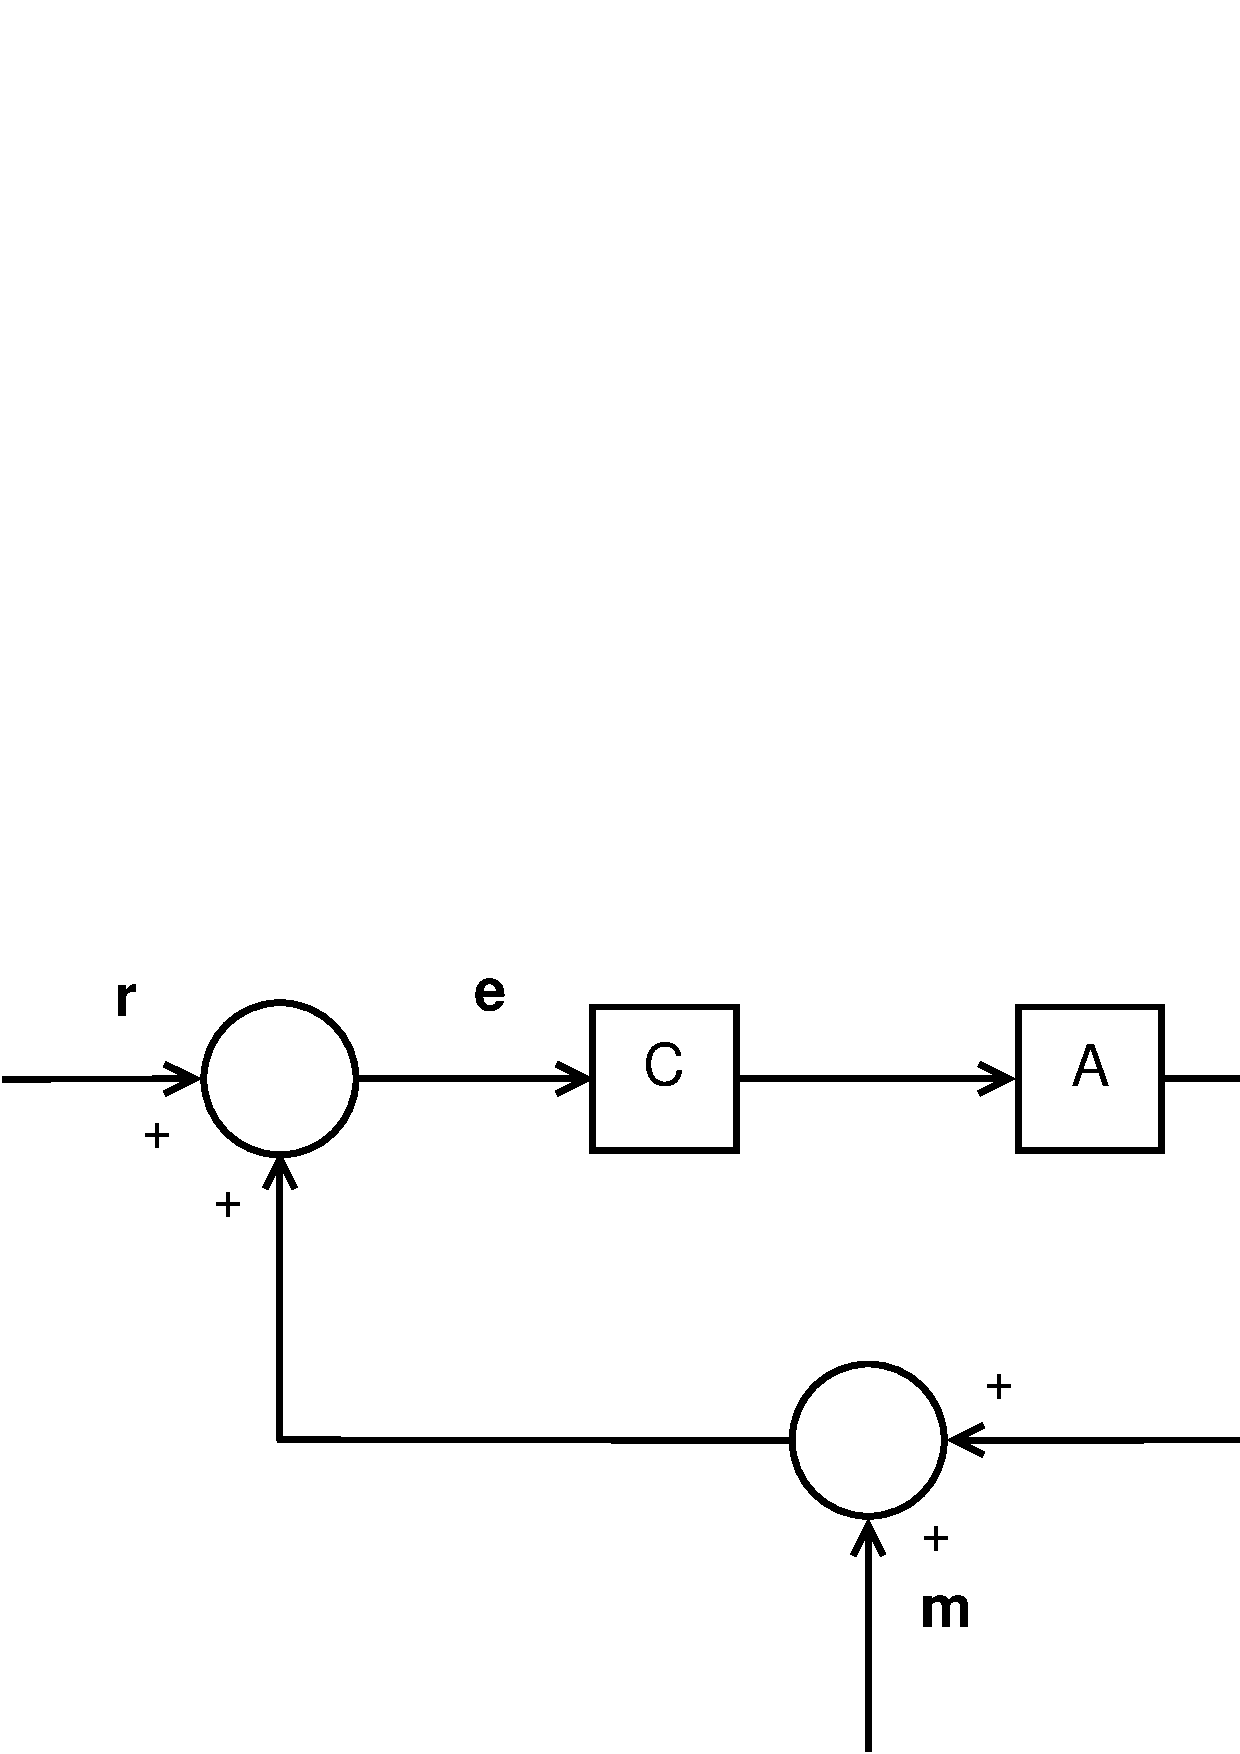
\includegraphics[width=1\linewidth]{full_system1}
\end{figure}
\end{frame}

%------------------------------------------------

\begin{frame}
\vspace{-4ex}
\frametitle{Control theory}
\begin{figure}
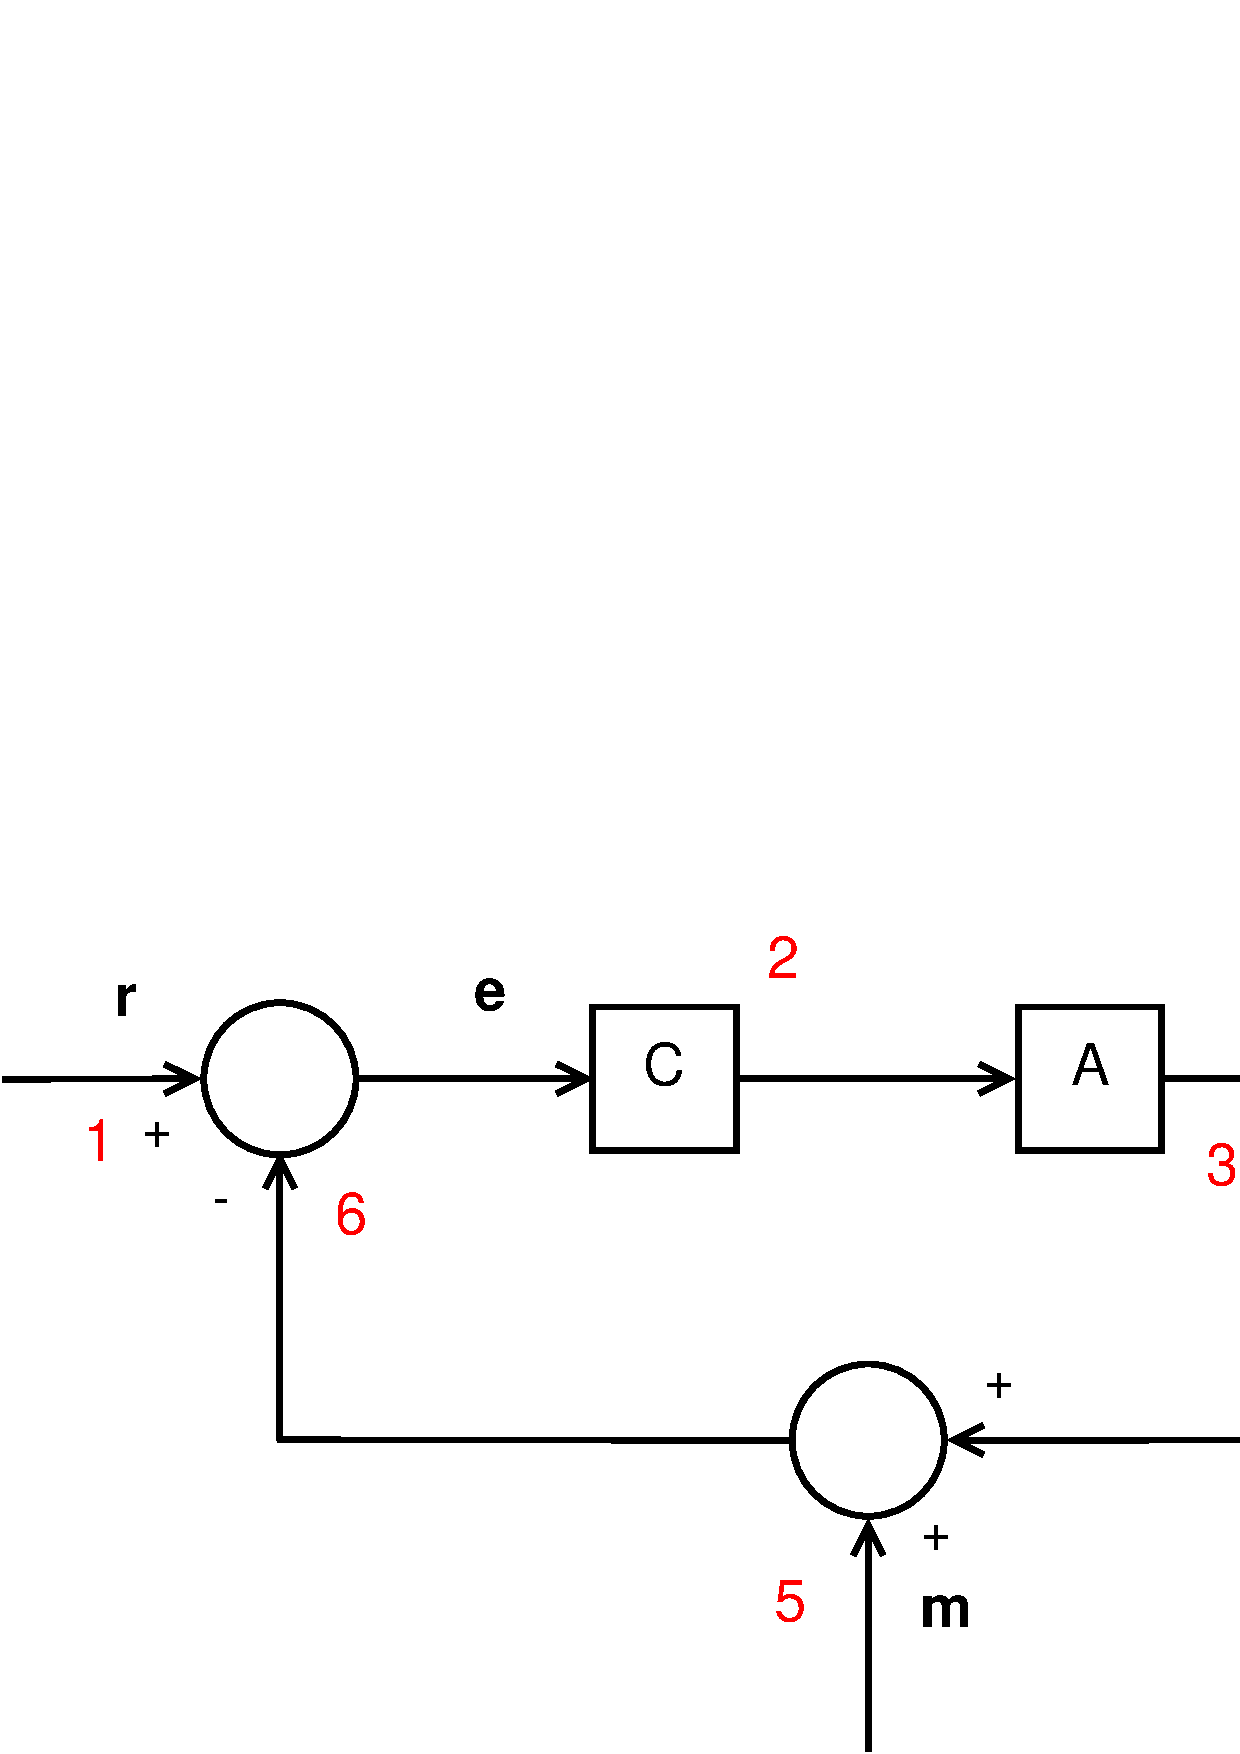
\includegraphics[width=1\linewidth]{full_system2}
\end{figure}
\vspace{-4ex}
1. reference signals: the desired output signals\\
2. controller with model (controller = dynamic)\\
3. actuators that control the system\\
4. Noise\\
5. Measurement noise\\
6. Negative feedback $\rightarrow$ system = stable 
\end{frame}

%------------------------------------------------

\begin{frame}
\frametitle{Example}
\vspace{-11ex}
Speed control system\\
\bigskip
\bigskip
\begin{figure}
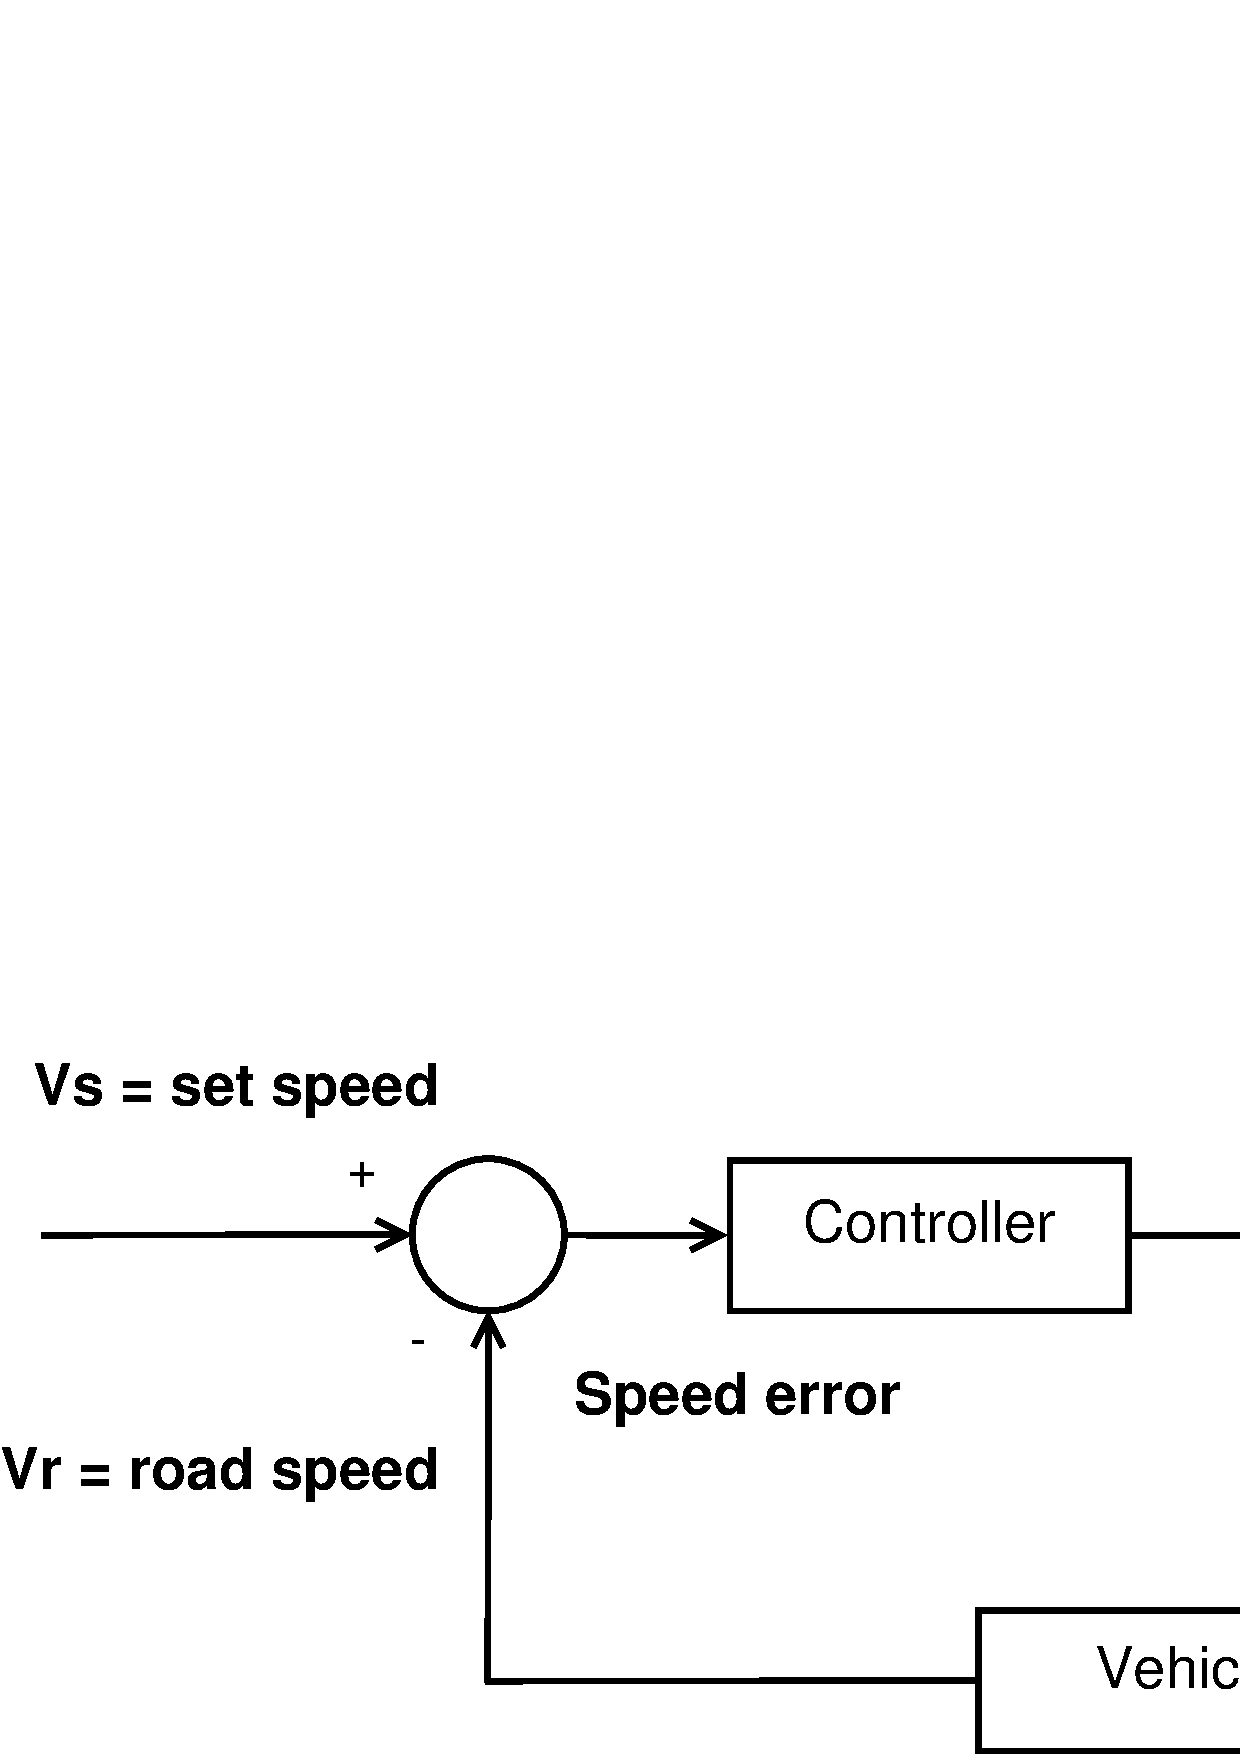
\includegraphics[width=1\linewidth]{speed_control_system}
\end{figure}
\end{frame}

%------------------------------------------------

\begin{frame}
\frametitle{Example}
\vspace{-6ex}
Temperature control system\\
\bigskip
\begin{figure}
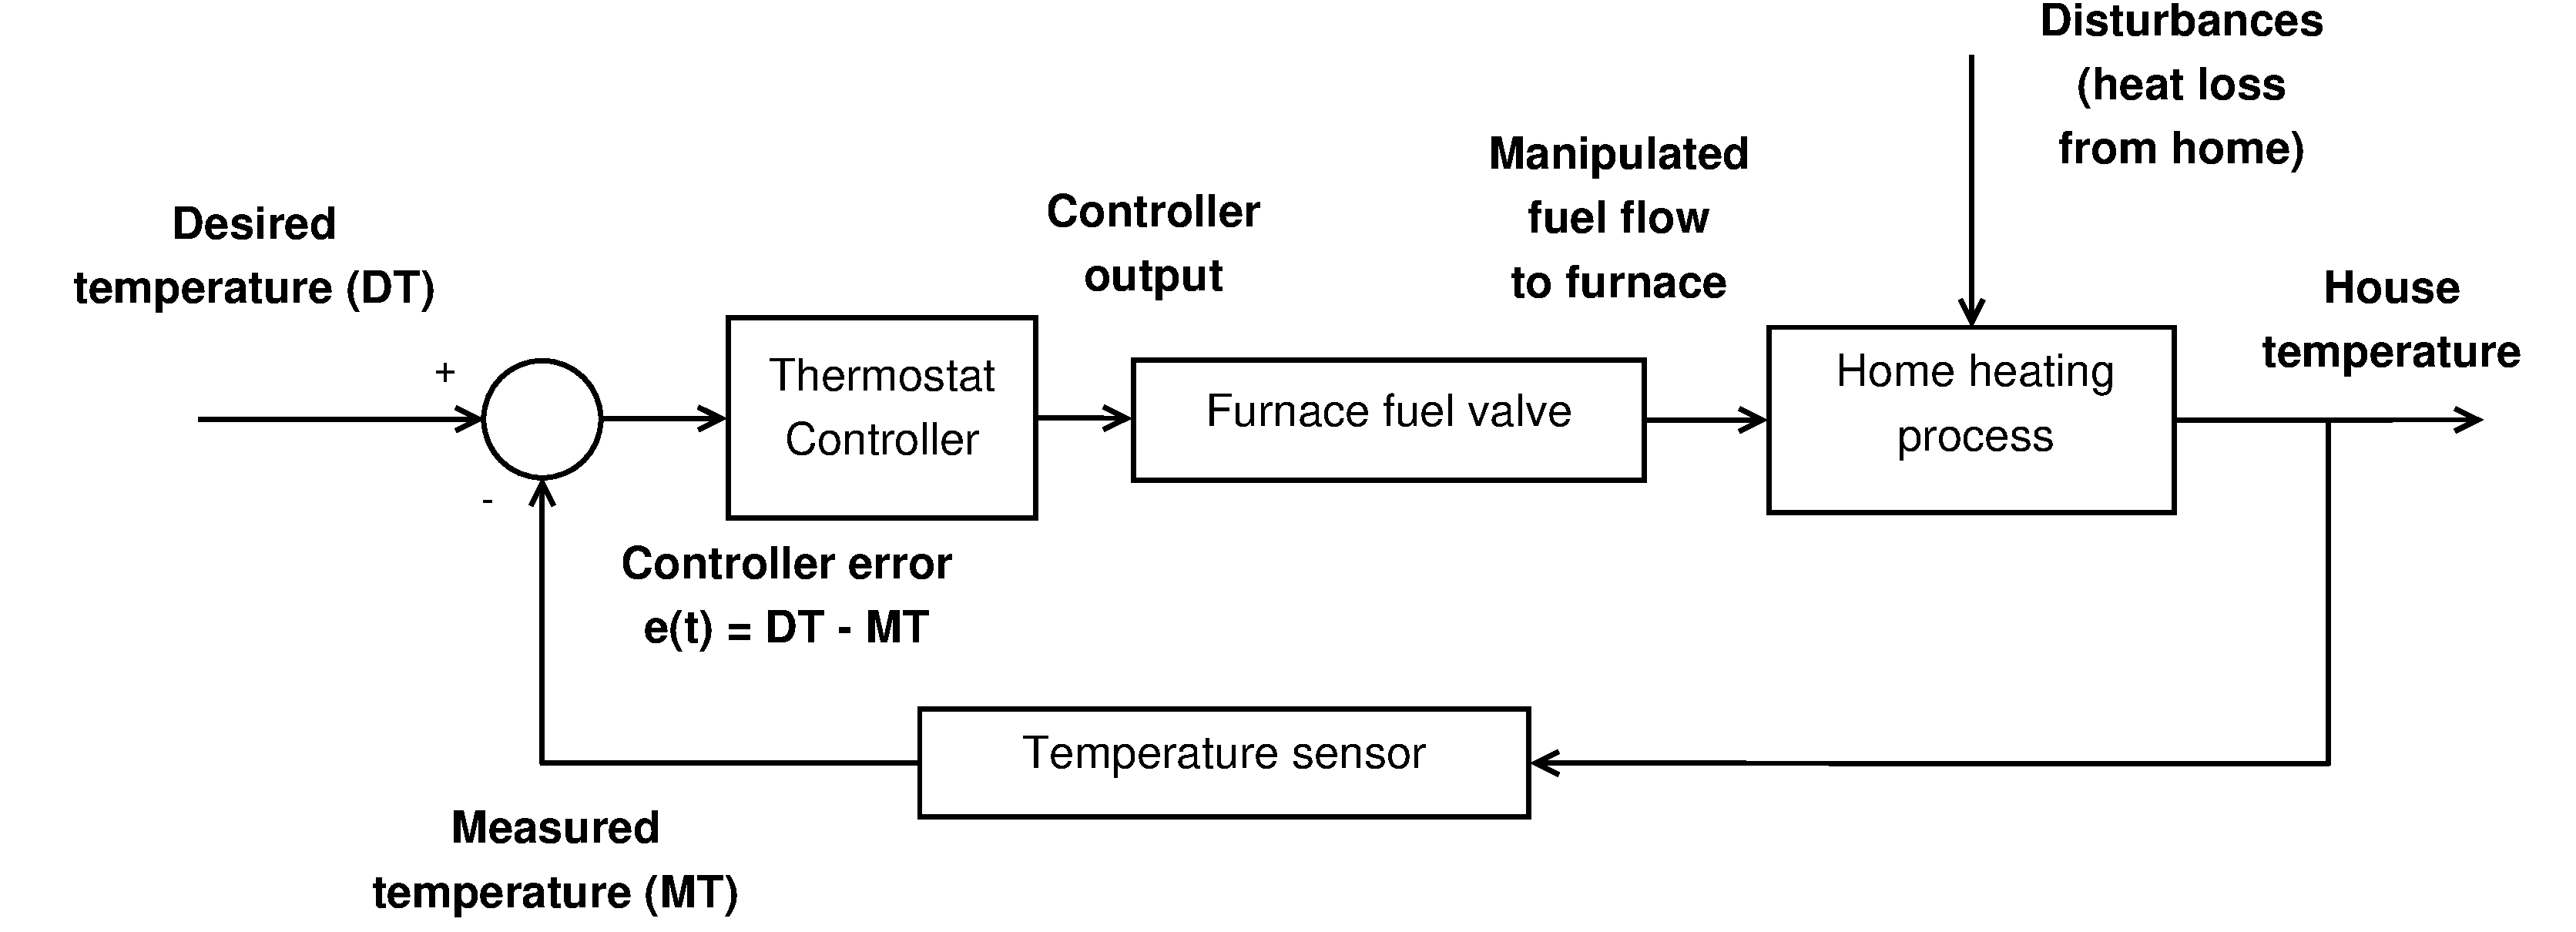
\includegraphics[width=1\linewidth]{temp_control_system}
\end{figure}
\end{frame}

%------------------------------------------------

\begin{frame}
\frametitle{Automation}
\begin{figure}

\includegraphics[width=1\linewidth]{automation}
\end{figure}
\url{https://youtu.be/XJLMW6l303g}
\end{frame}

%------------------------------------------------
\section{Open-loop vs. closed-loop systems} 
%------------------------------------------------

\begin{frame}
\frametitle{Open loop}
\vspace{-10ex}
In an open loop system, the output is not fed back into the controller. Therefore, the controller cannot \textit{'see'} the effect of its actions. \\
This way it is hard to get the desired output.\\
\bigskip
\bigskip
\begin{figure}
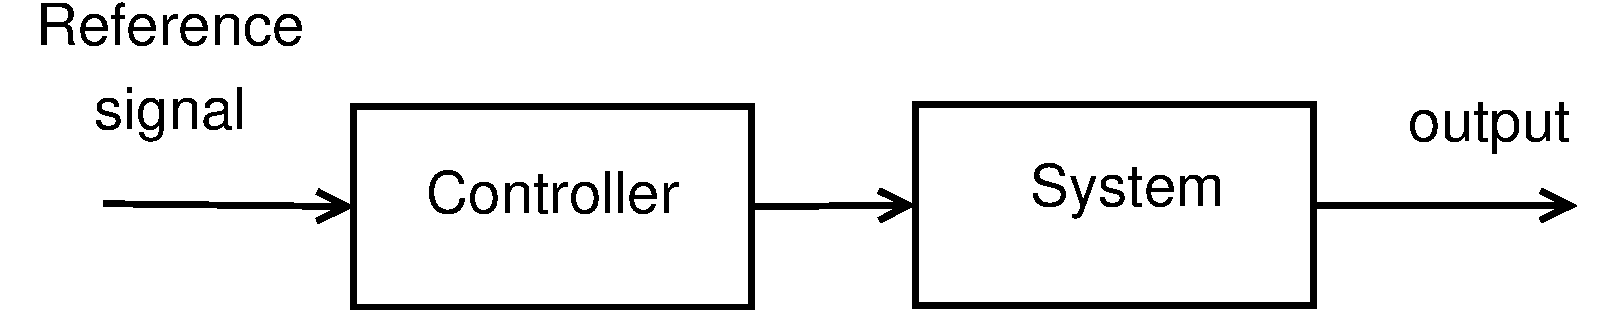
\includegraphics[width=1\linewidth]{open_loop}
\end{figure}
\end{frame}

%------------------------------------------------

\begin{frame}
\frametitle{Open loop}
\begin{columns}[c]

\column{.5\textwidth}
Take for example the following system:\\
\begin{itemize}
\item You are pouring a glass of water, but you \textbf{cannot look at the glass}.
\item You know the desired output is a full glass of water within a reasonable time.
\item The input can have two values: on or off (assume you are using a quite primitive tap).
\item You can imagine it will not be easy to do this successfully.
\end{itemize}

\column{.5\textwidth}
\begin{figure}
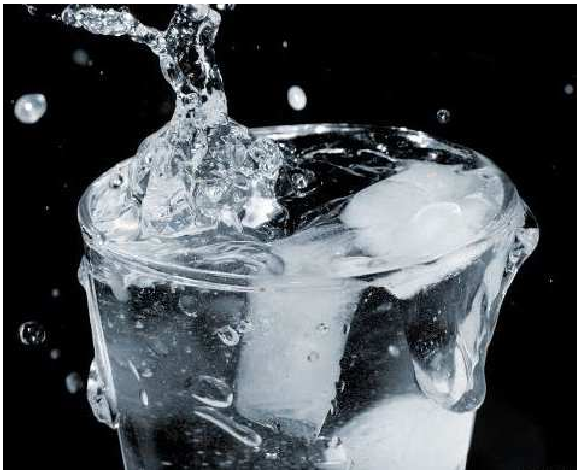
\includegraphics[width=1\linewidth]{glass}
\end{figure}

\end{columns}
\bigskip
The solution is evident: look at the glass while pouring!
\end{frame}

%------------------------------------------------

\begin{frame}
\frametitle{Closed loop}
\vspace{-4ex}
In a closed loop system, the actuating error signal, which is the difference between the input signal and the feedback, is fed to the controller so as to reduce the error and bring the output to the desired value. 
\medskip
\begin{figure}
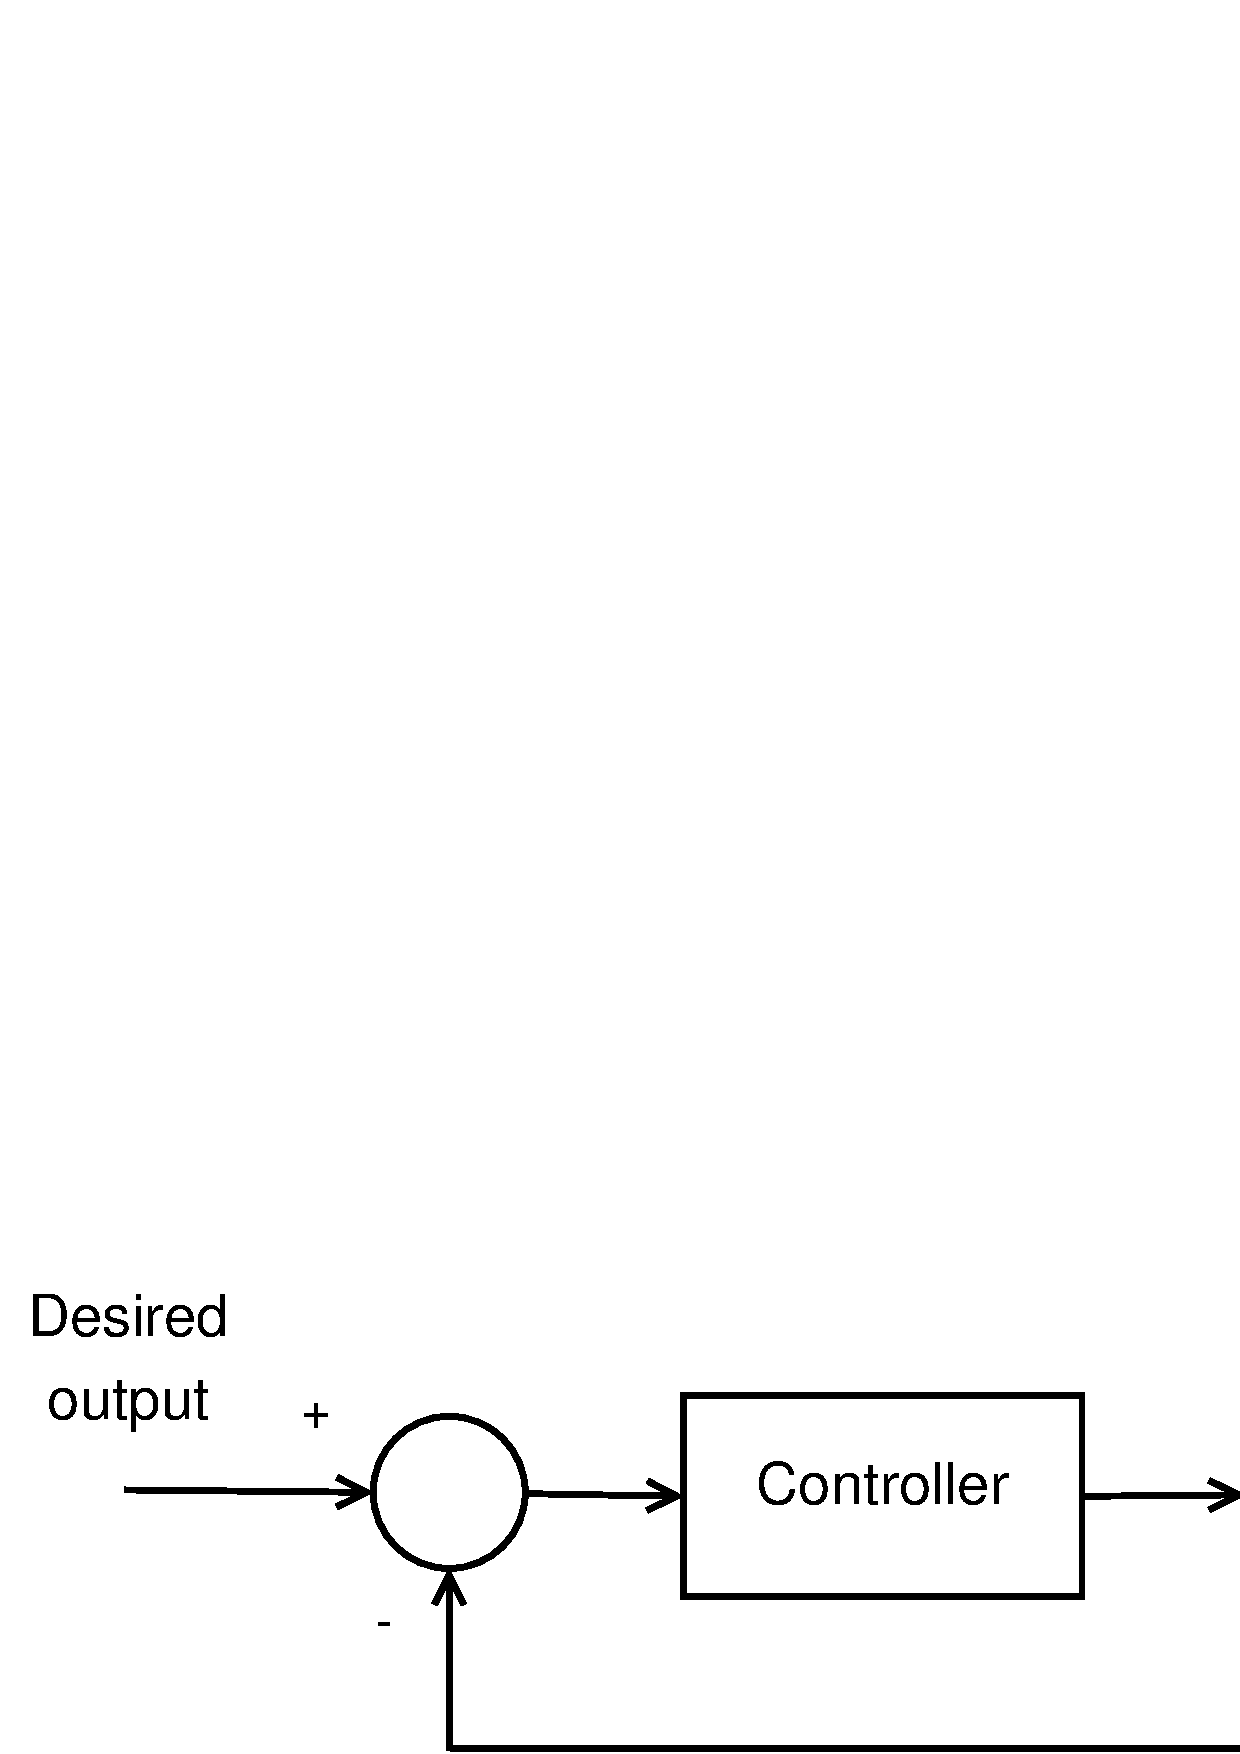
\includegraphics[width=1\linewidth]{closed_loop}
\end{figure}
\bigskip
Closed-loop always implies the use of feedback control.
\end{frame}

%------------------------------------------------
\section{Feedback} 
%------------------------------------------------

\begin{frame}
\frametitle{Feedback}
Feedback systems maintain the prescribed relationship between the output and the reference input by comparing them and using their difference.
\medskip
\begin{figure}
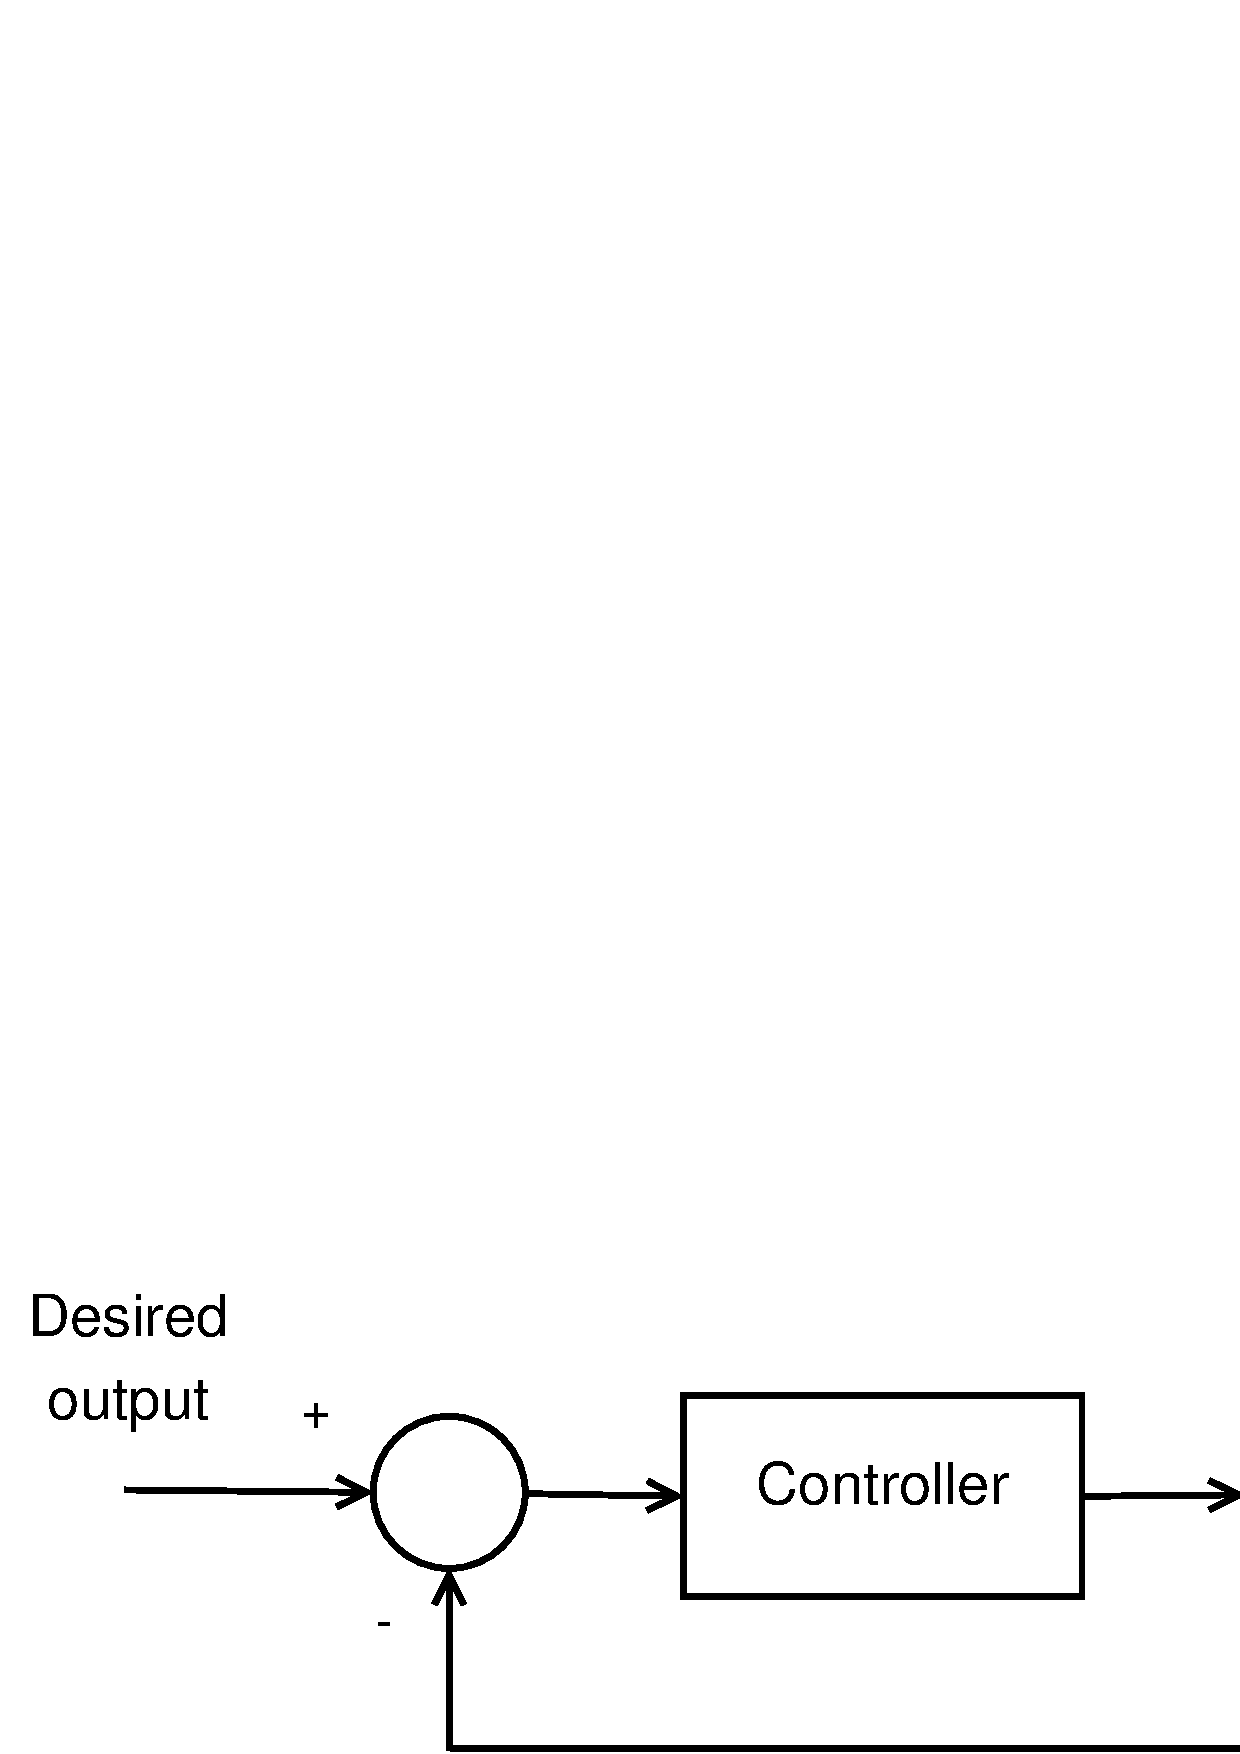
\includegraphics[width=1\linewidth]{closed_loop}
\end{figure}
There are two types of feedback systems. The output can either be added to the reference input (positive feedback) or substracted from it (negative feedback).\\
\medskip
\textit{Slides courtesy of prof. Rodolphe Sepulchre}
\end{frame}

%------------------------------------------------

\begin{frame}
\frametitle{Range-localized sensitivity is a nonlinear behavior}
\center{\Large{$V = sat(I)$}}
\begin{figure}
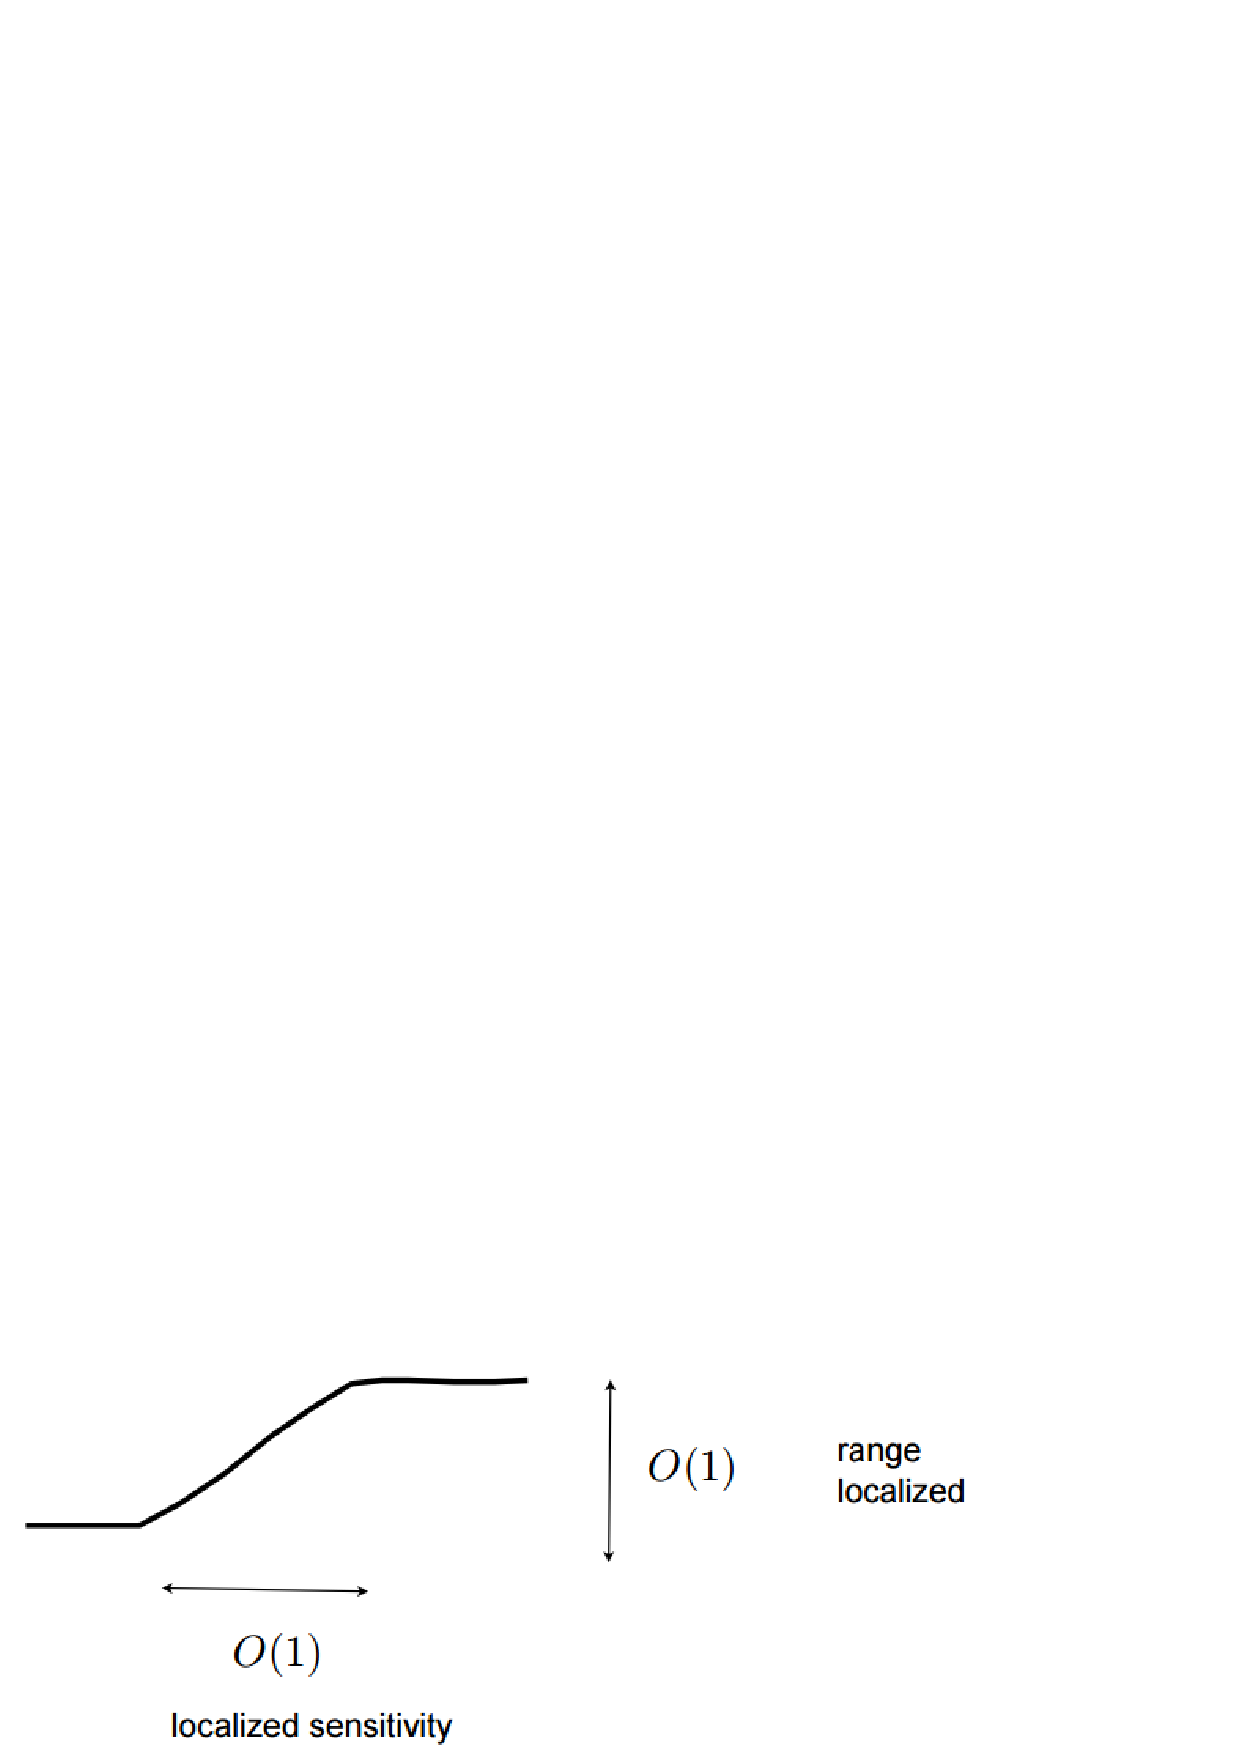
\includegraphics[width=1\linewidth]{range_localization}
\end{figure}
\end{frame}

%------------------------------------------------

\begin{frame}
\frametitle{Black principle: negative feedback 'linearizes'}
\begin{figure}
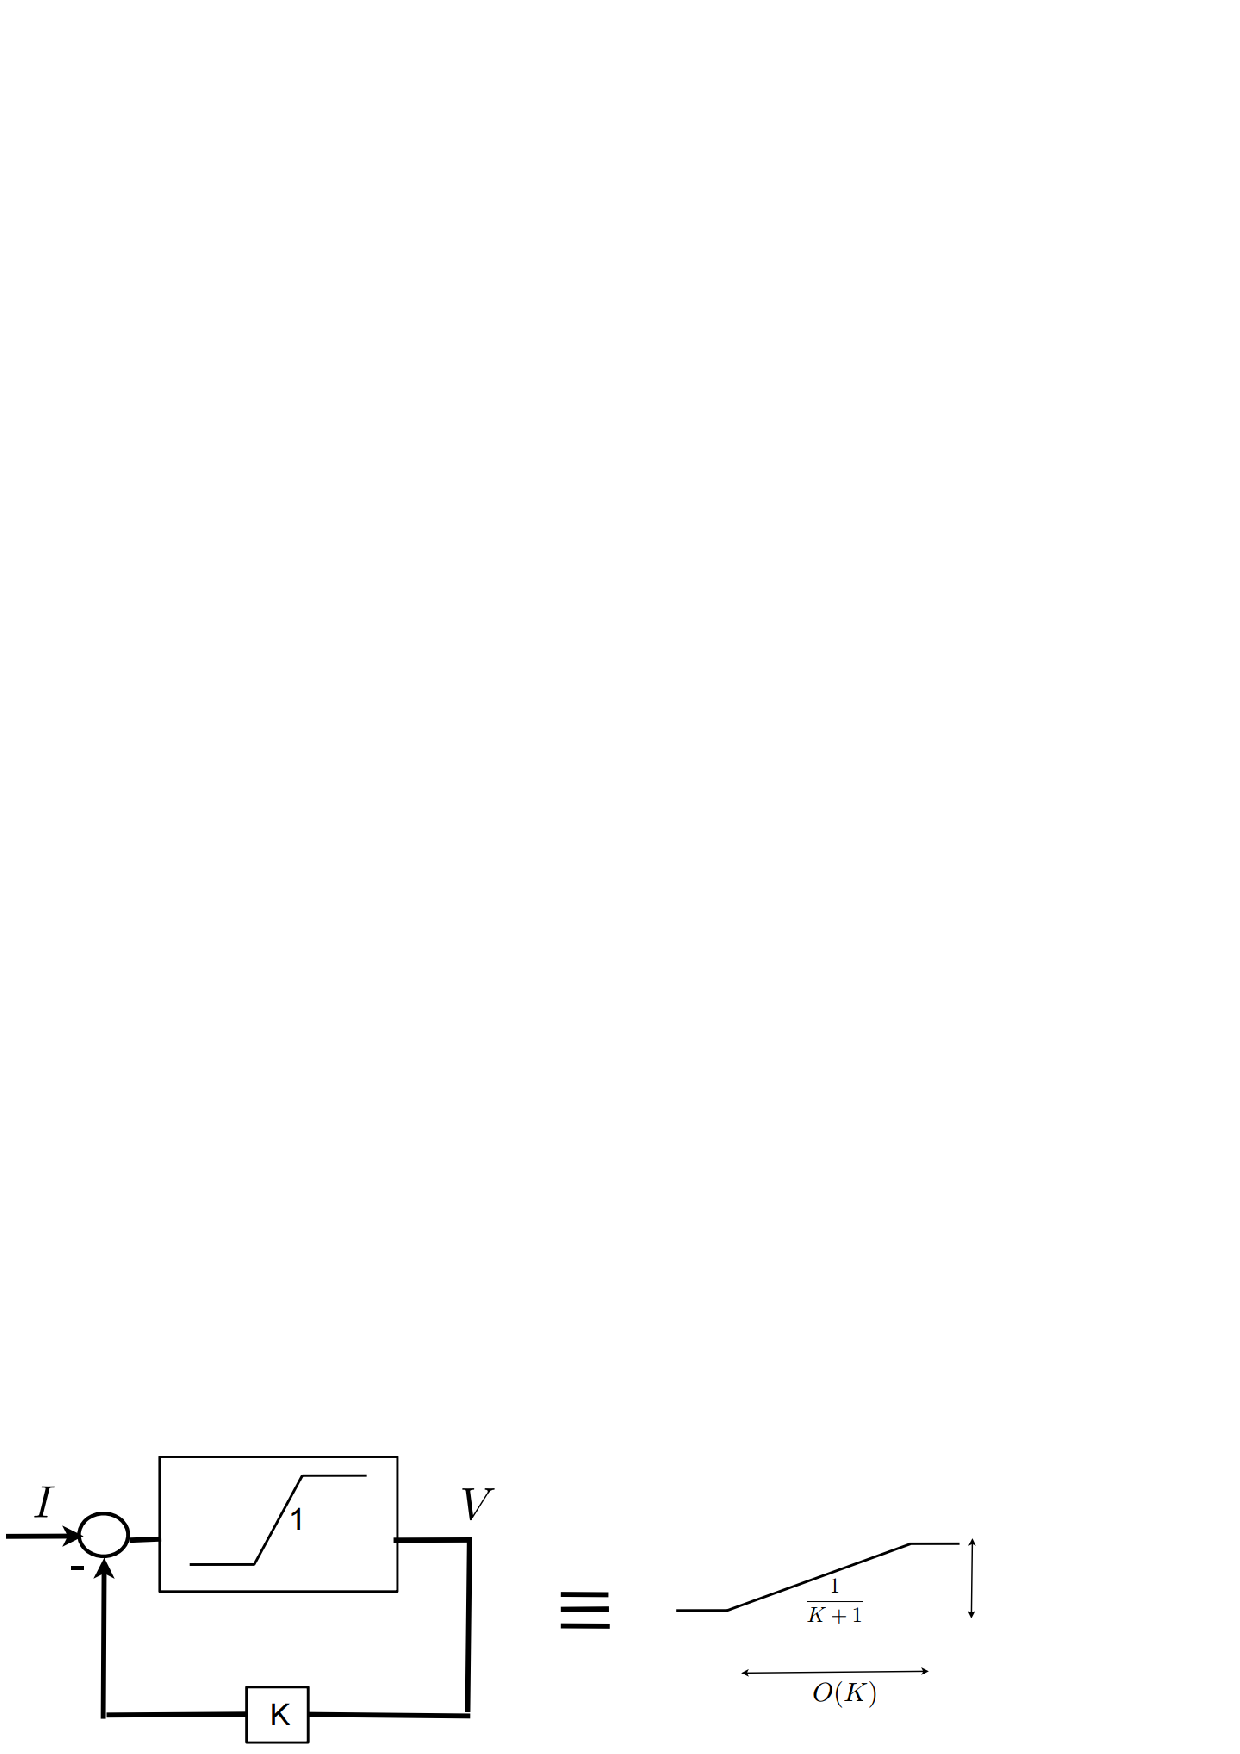
\includegraphics[width=1\linewidth]{black_negative}
\end{figure}
\begin{center}
$V = sat_{1}(I - KV) \equiv V = sat_{\frac{1}{1+K}}(I)$\\
\end{center}
\medskip
Sensitivity domain is spread by negative feedback\\
(The essence of control theory)
\end{frame}

%------------------------------------------------

\begin{frame}
\frametitle{Black principle: positive feedback 'quantizes'}
\begin{figure}
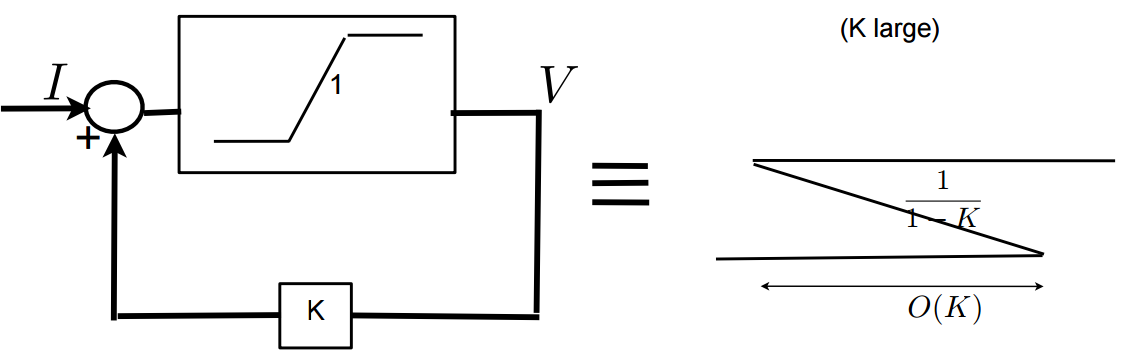
\includegraphics[width=1\linewidth]{black_positive}
\end{figure}
\[   
V =  sat_{1}(I + KV) \equiv V =
     \begin{cases}
       \mbox{+1} &\quad \text{$I \geq -1-K$}\\
       \mbox{-1} &\quad \text{$I \leq K-1$}\
     \end{cases}
\]
Sensitivity domain is spread by negative feedback\\
$\;$
\end{frame}

%------------------------------------------------

\begin{frame}
\frametitle{Black feedback principle}
\vspace{-2ex}
\begin{columns}[c]

\column{.5\textwidth}
\begin{figure}
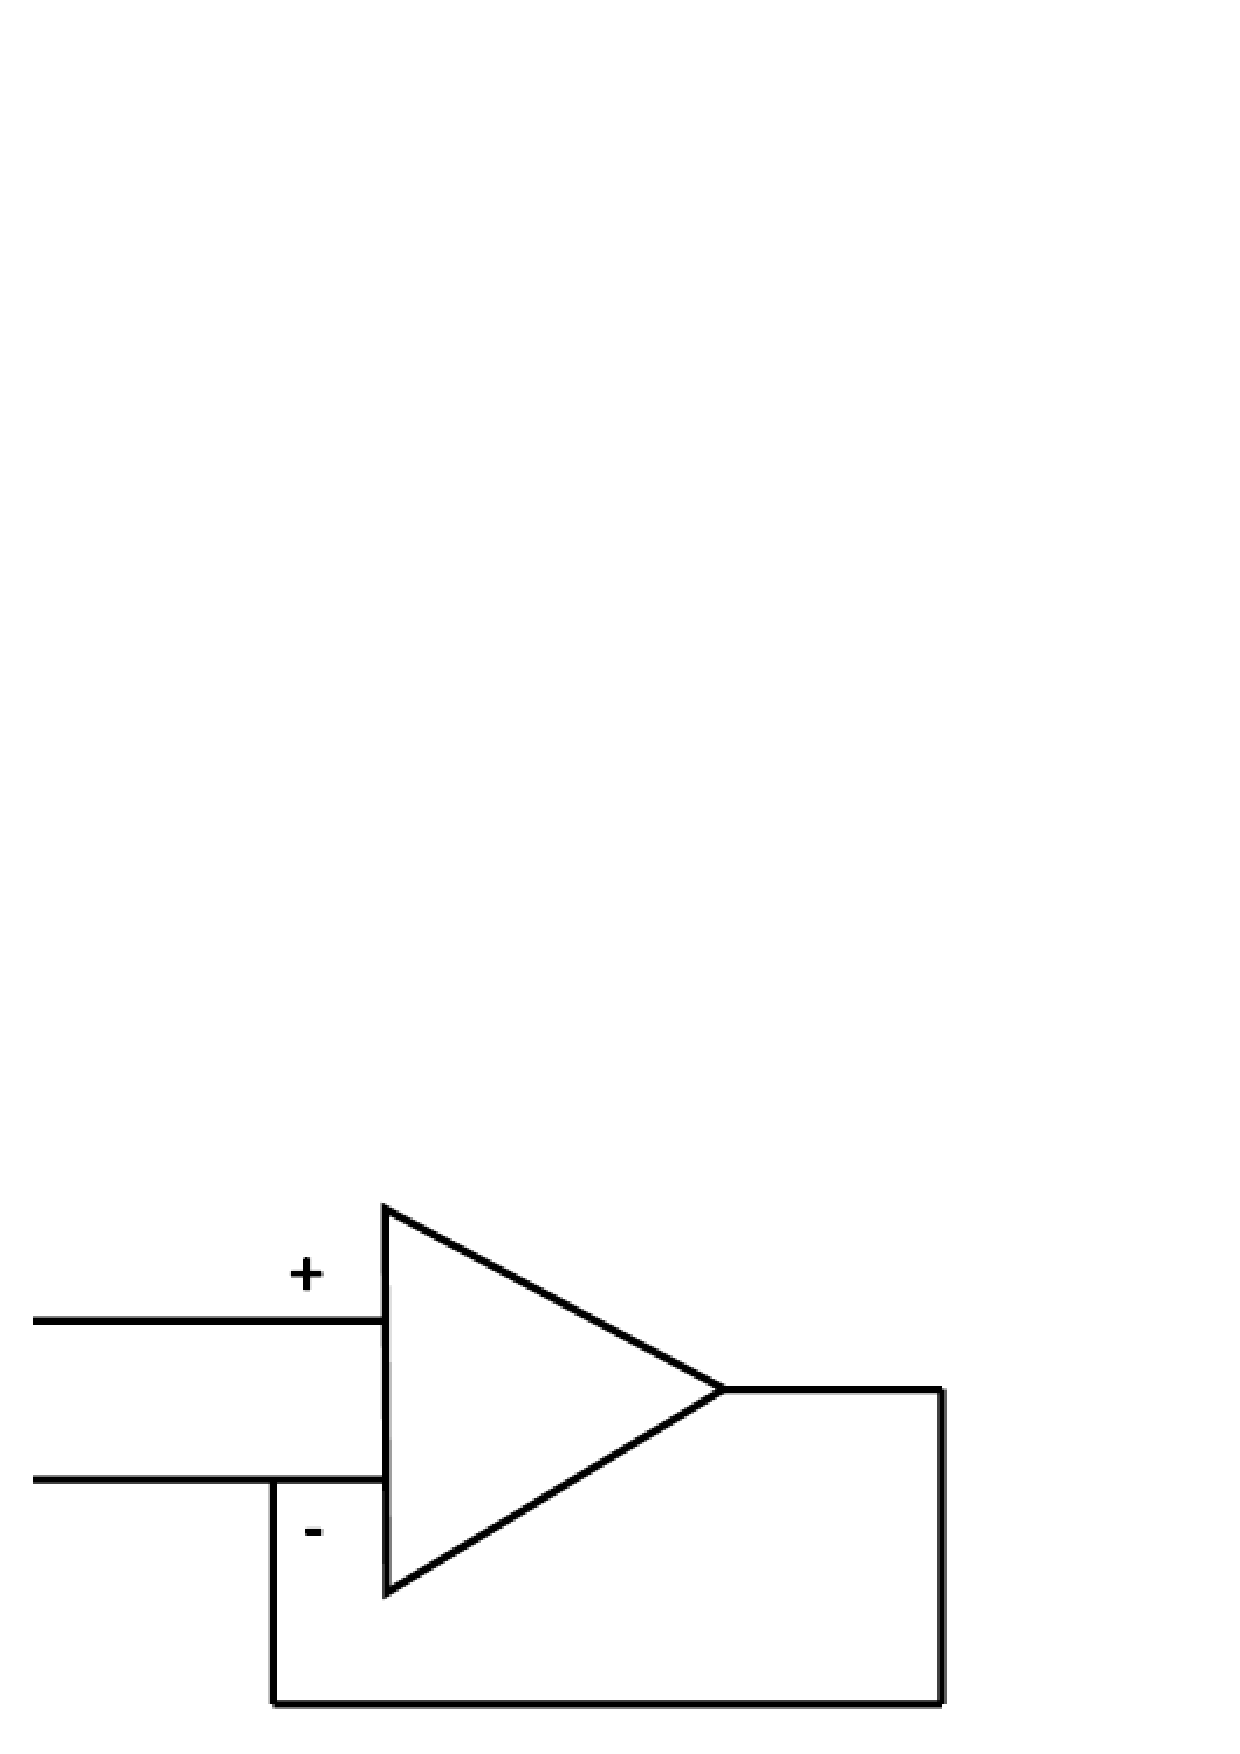
\includegraphics[width=1\linewidth]{negative}
\end{figure}
\vspace{-4ex}
\begin{enumerate}
\item Negative feedback linearizes
\item Continuous behavior
\item Analog technology
\item Output primarily reflects the input
\item Loops enhance or amplify the changes between input and output
\end{enumerate}

\column{.5\textwidth}
\begin{figure}
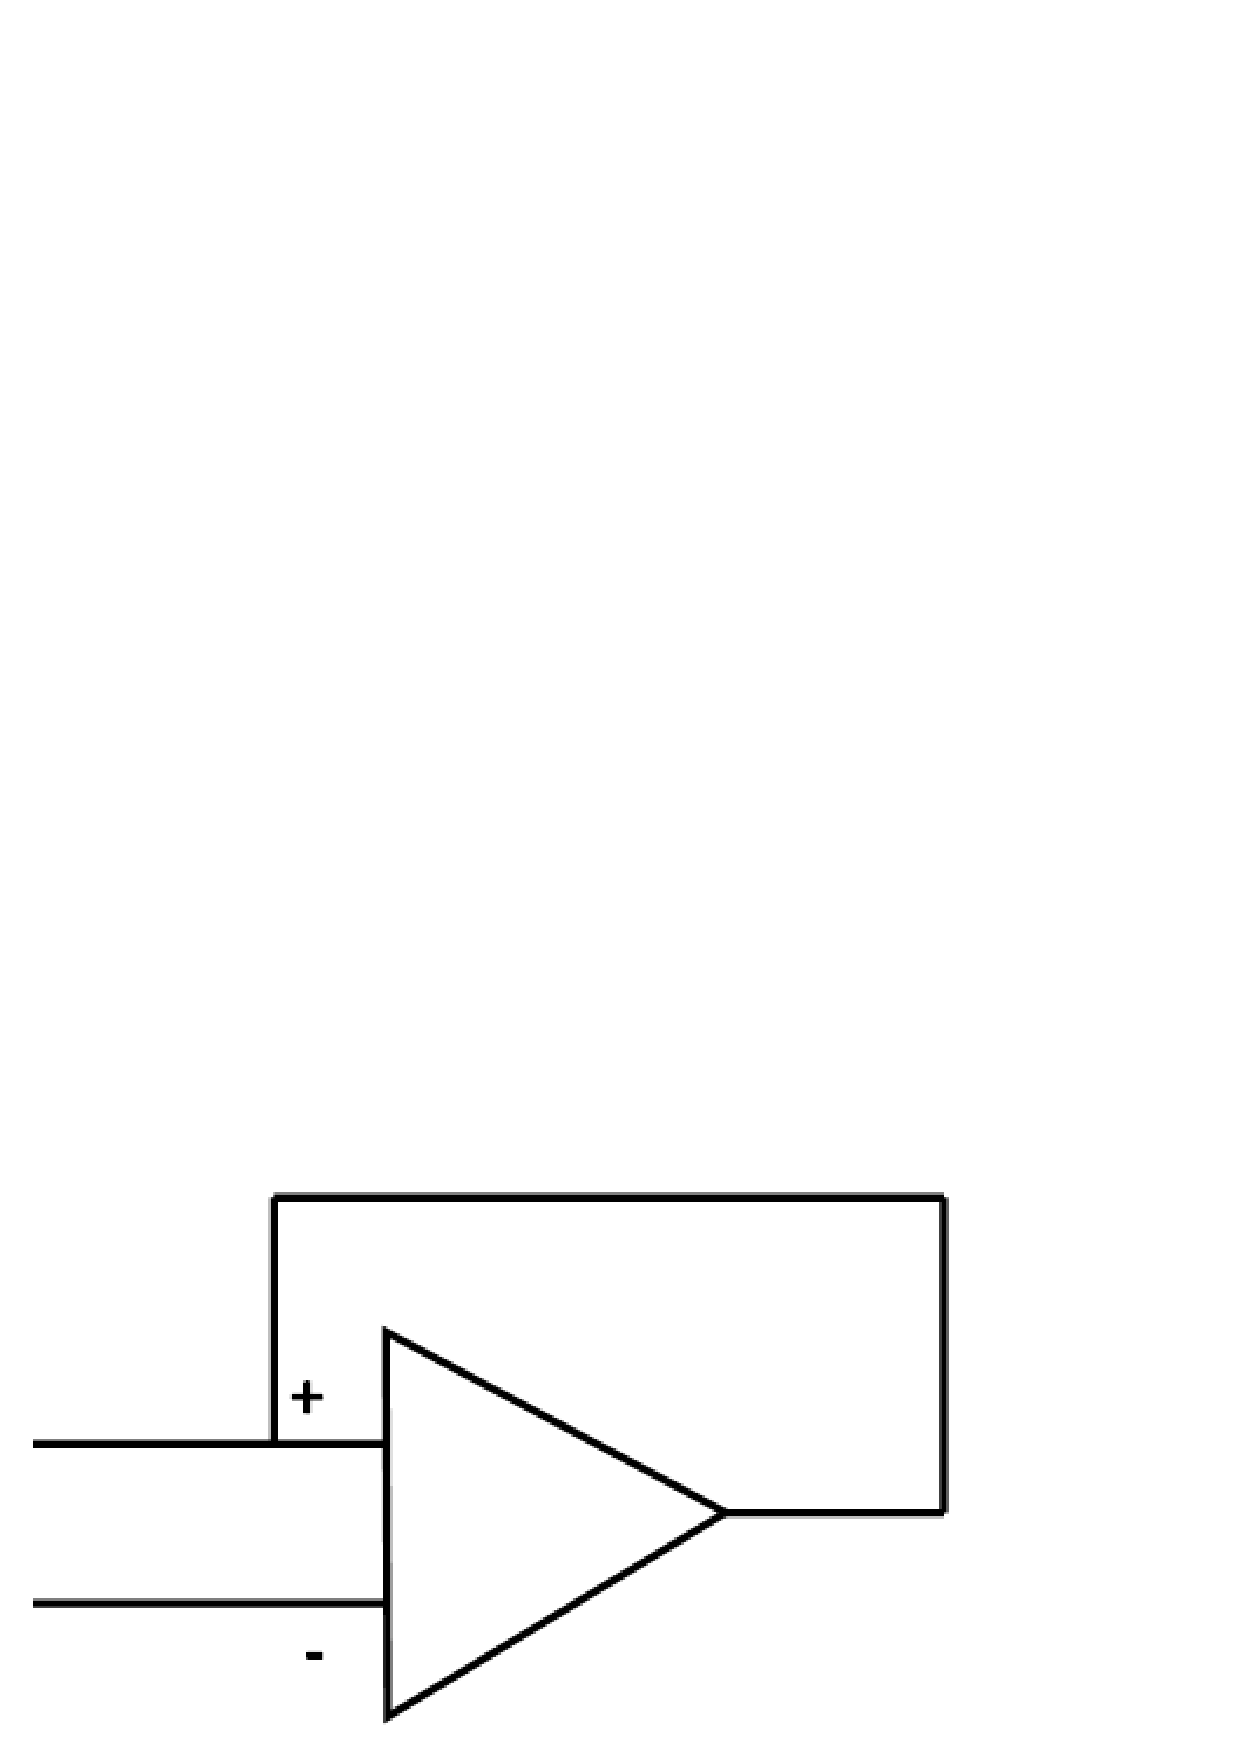
\includegraphics[width=1\linewidth]{positive}
\end{figure}
\vspace{-4ex}
\begin{enumerate}
\item Positive feedback quantizes
\item On-Off behavior
\item Digital Technology
\item Output primarily reflects memory of the past
\item Loops tend to dampen or buffer the changes between input and output
\end{enumerate}

\end{columns}
\end{frame}

%------------------------------------------------

\begin{frame}
\frametitle{Balanced feedback 'localizes'}
\vspace{-2ex}
\begin{columns}[c]

\column{.3\textwidth}
\begin{figure}
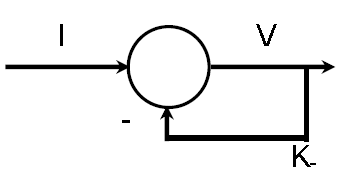
\includegraphics[width=1\linewidth]{linear}
\end{figure}
\center{\textit{\Large{'linear'}}}\\
\center{$|k| large$}

\column{.3\textwidth}
\begin{figure}
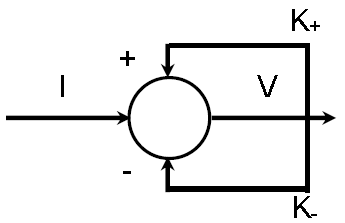
\includegraphics[width=1\linewidth]{localized}
\end{figure}
\vspace{-5ex}
\center{\textit{\Large{'localized'}}}\\
\center{$|k| small$}

\column{.3\textwidth}
\begin{figure}
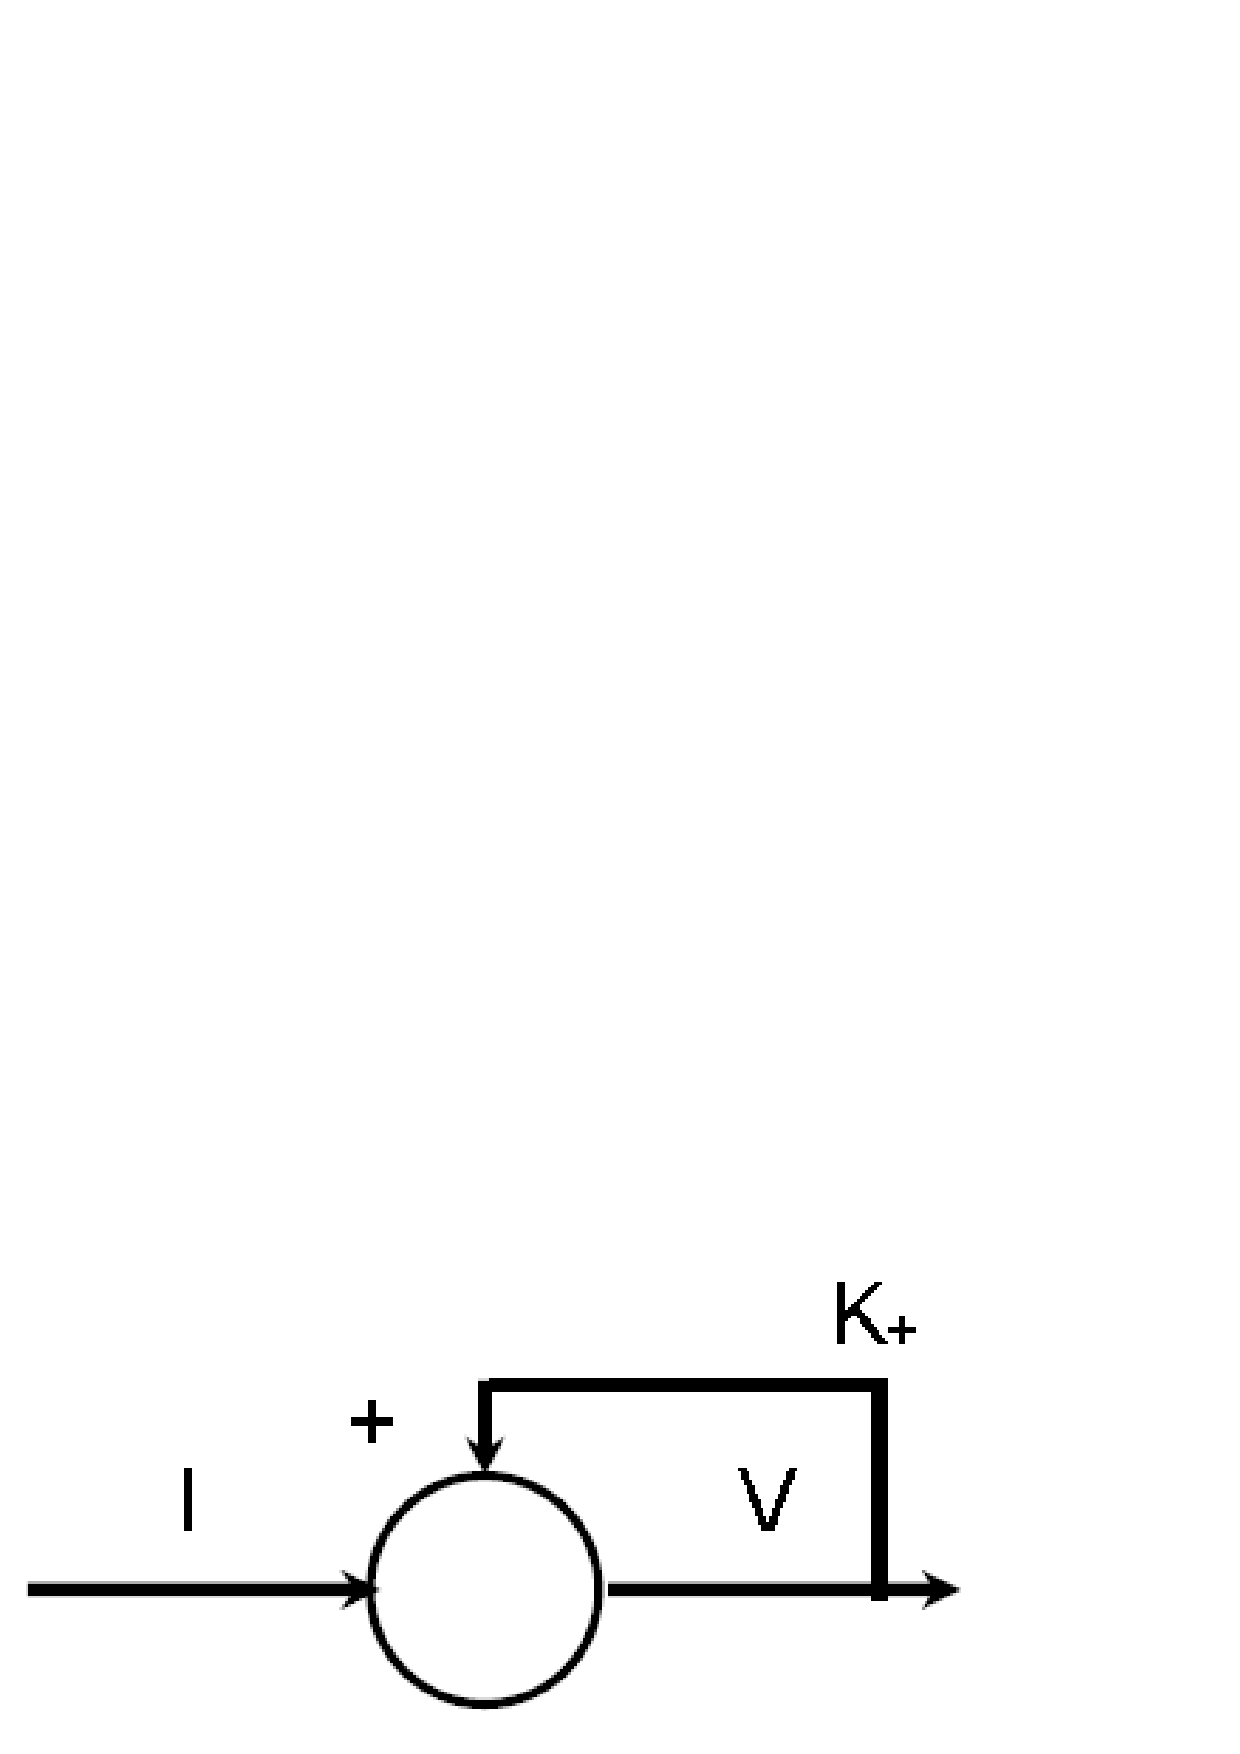
\includegraphics[width=1\linewidth]{memory}
\end{figure}
\center{\textit{\Large{'memory'}}}\\
\center{$|k| large$}

\end{columns}
\begin{figure}
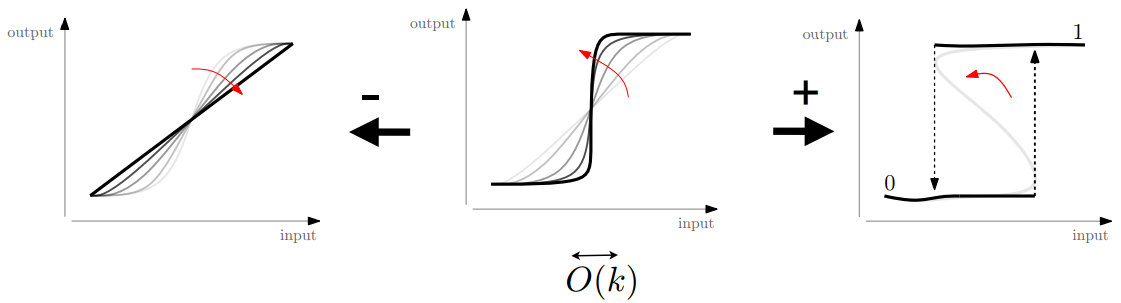
\includegraphics[width=1\linewidth]{balanced_feedback}
\end{figure}
\vspace{-2ex}
\center{$k \approx K_{+} - K_{-}$}
\end{frame}

%------------------------------------------------

\begin{frame}
\frametitle{Robust space + time localization by feedback}
\begin{figure}
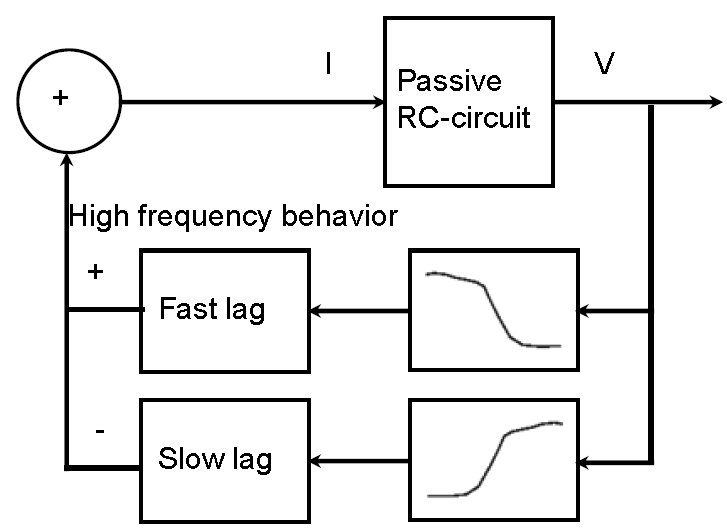
\includegraphics[width=.7\linewidth]{robust}
\end{figure}
Low frequency behavior\\
Necessary localization in same frequency range!
\end{frame}

%------------------------------------------------

\begin{frame}
\frametitle{Guitar feedback}
\begin{figure}
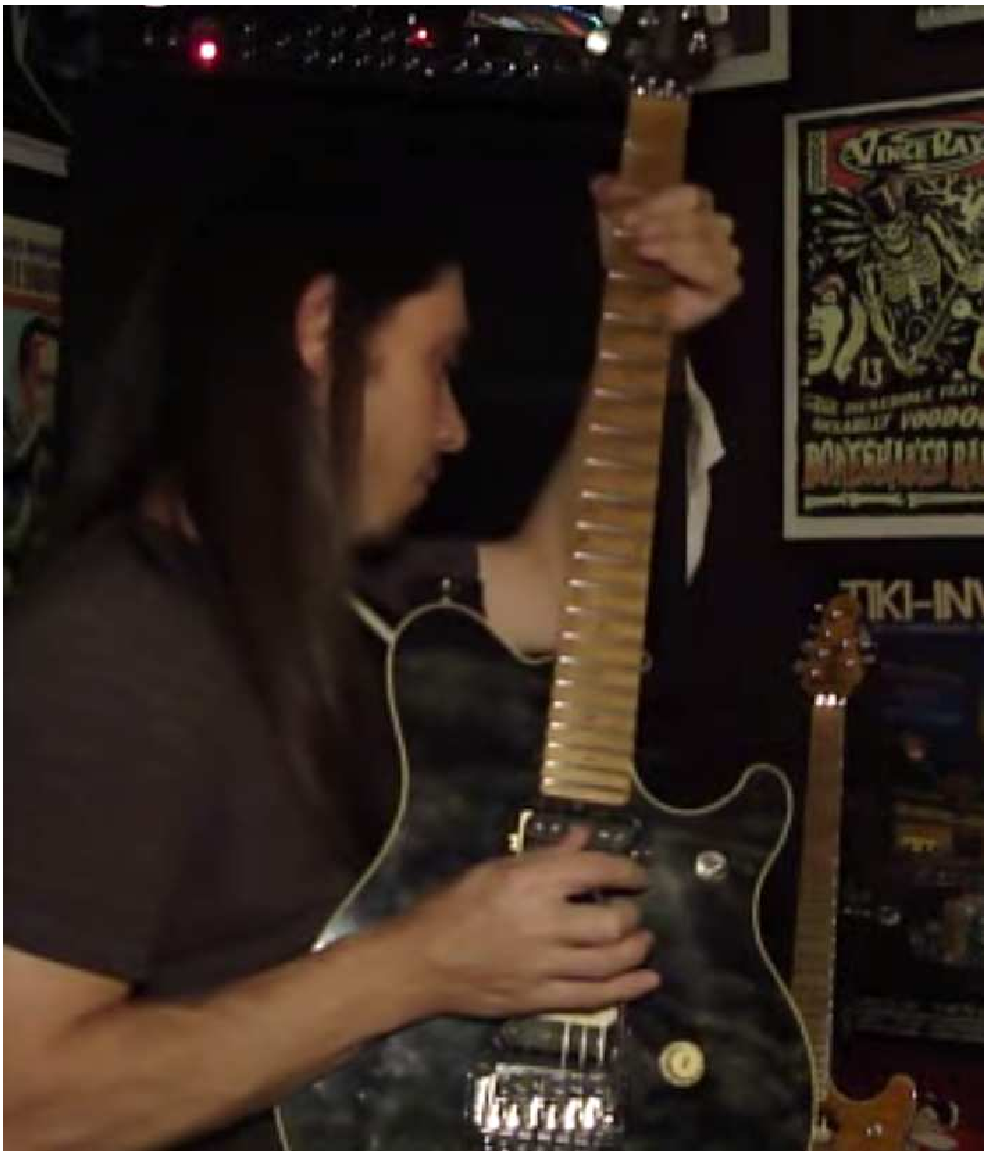
\includegraphics[width=.5\linewidth]{guitar}
\end{figure}
\url{https://youtu.be/luURyH9fzhk}
\end{frame}

%------------------------------------------------

\begin{frame}
\frametitle{What if there was no feedback?}
\begin{figure}
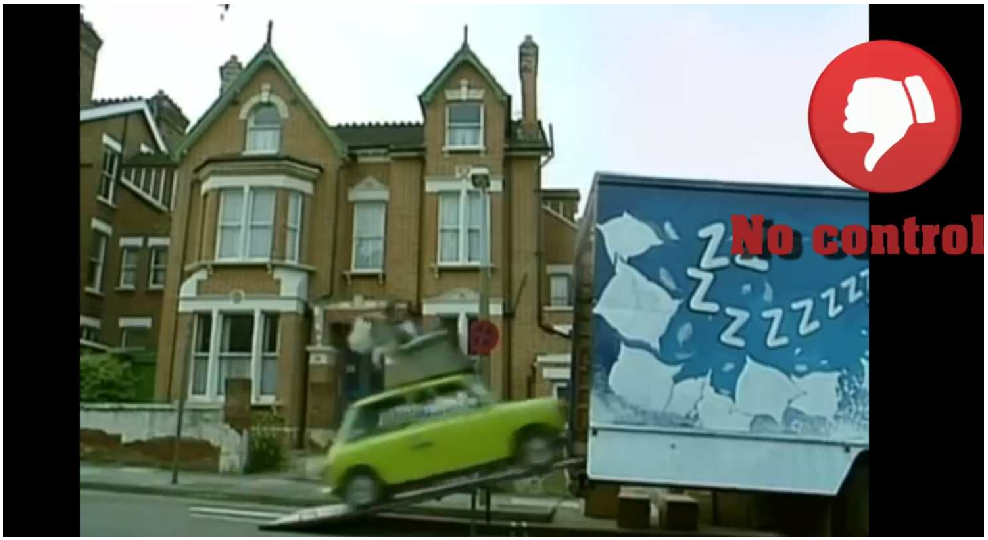
\includegraphics[width=1\linewidth]{no_feedback}
\end{figure}
\bigskip
\url{https://youtu.be/C221sI1W9Gk}
\end{frame}

%------------------------------------------------

\begin{frame}
\frametitle{Feedback loops in biology}
\begin{figure}
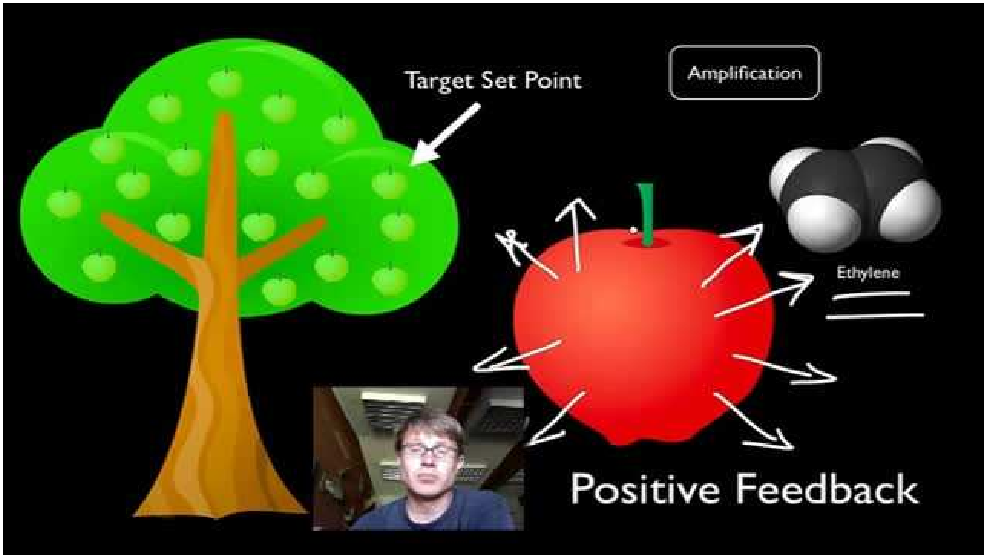
\includegraphics[width=1\linewidth]{feedback_biology}
\end{figure}
\bigskip
\url{https://www.youtube.com/watch?v=CLv3SkF_Eag}
\end{frame}

%------------------------------------------------

%\begin{frame}
%\frametitle{Types of controllers}
%
%\vspace{-4ex}
%\begin{figure}
%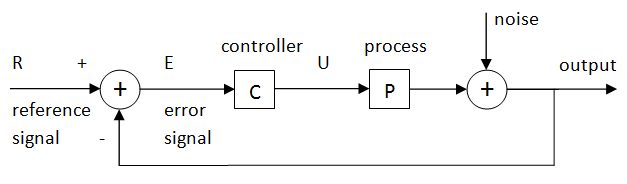
\includegraphics[width=.9\linewidth]{control_theory}
%\end{figure}
%\vspace{-4ex}
%\begin{columns}[c]
%
%\column{.5\textwidth}
%\textbf{Proportional controller}\\
%$C(s) = K$\\
%\medskip
%\textbf{Phase lead controller}\\
%$C(s) = K \frac{b}{a} \frac{s+a}{s+b} \qquad a<b$\\
%\medskip
%\textbf{Phase lag controller}\\
%$C(s) = K \frac{b}{a} \frac{s+a}{s+b} \qquad a>b$
%
%
%\column{.5\textwidth}
%\center \textbf{PID controller}\\
%\begin{figure}
%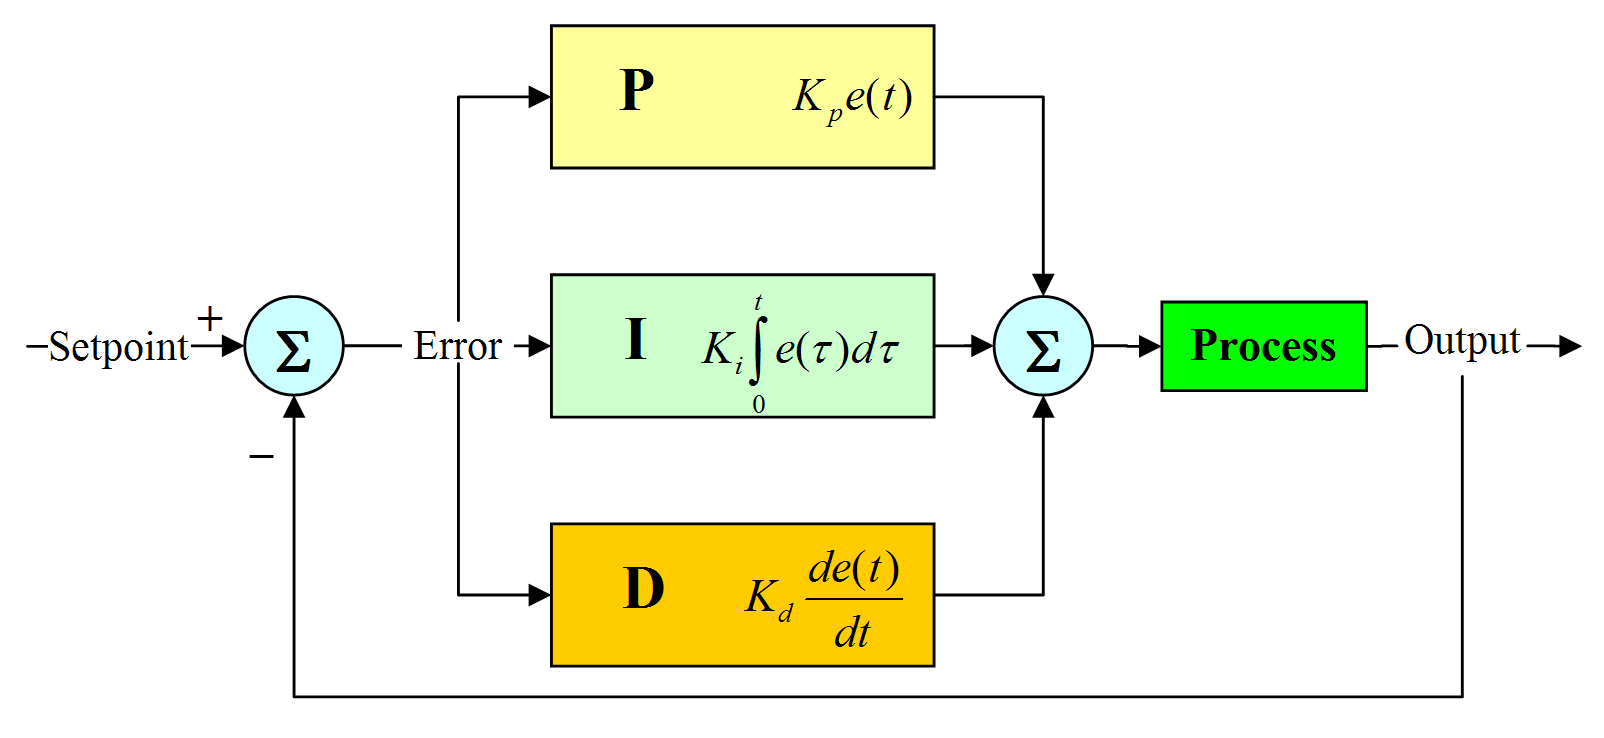
\includegraphics[width=1\linewidth]{PID}
%\end{figure}
%
%\end{columns}
%
%\end{frame}


%------------------------------------------------
\section{Automatic control} 
%------------------------------------------------

\begin{frame}
\frametitle{Dance of the Flying Machines}
\begin{figure}
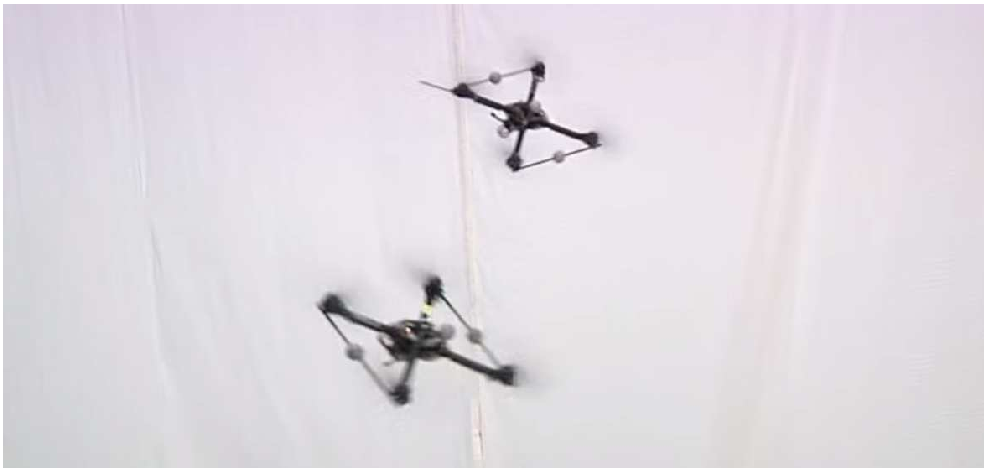
\includegraphics[scale=.7]{flying_machines}
\end{figure}
\url{https://youtu.be/NRL_1ozDQCA}
\end{frame}

%------------------------------------------------

\begin{frame}
\frametitle{Automated driving with precision at the physical limits}
\begin{figure}
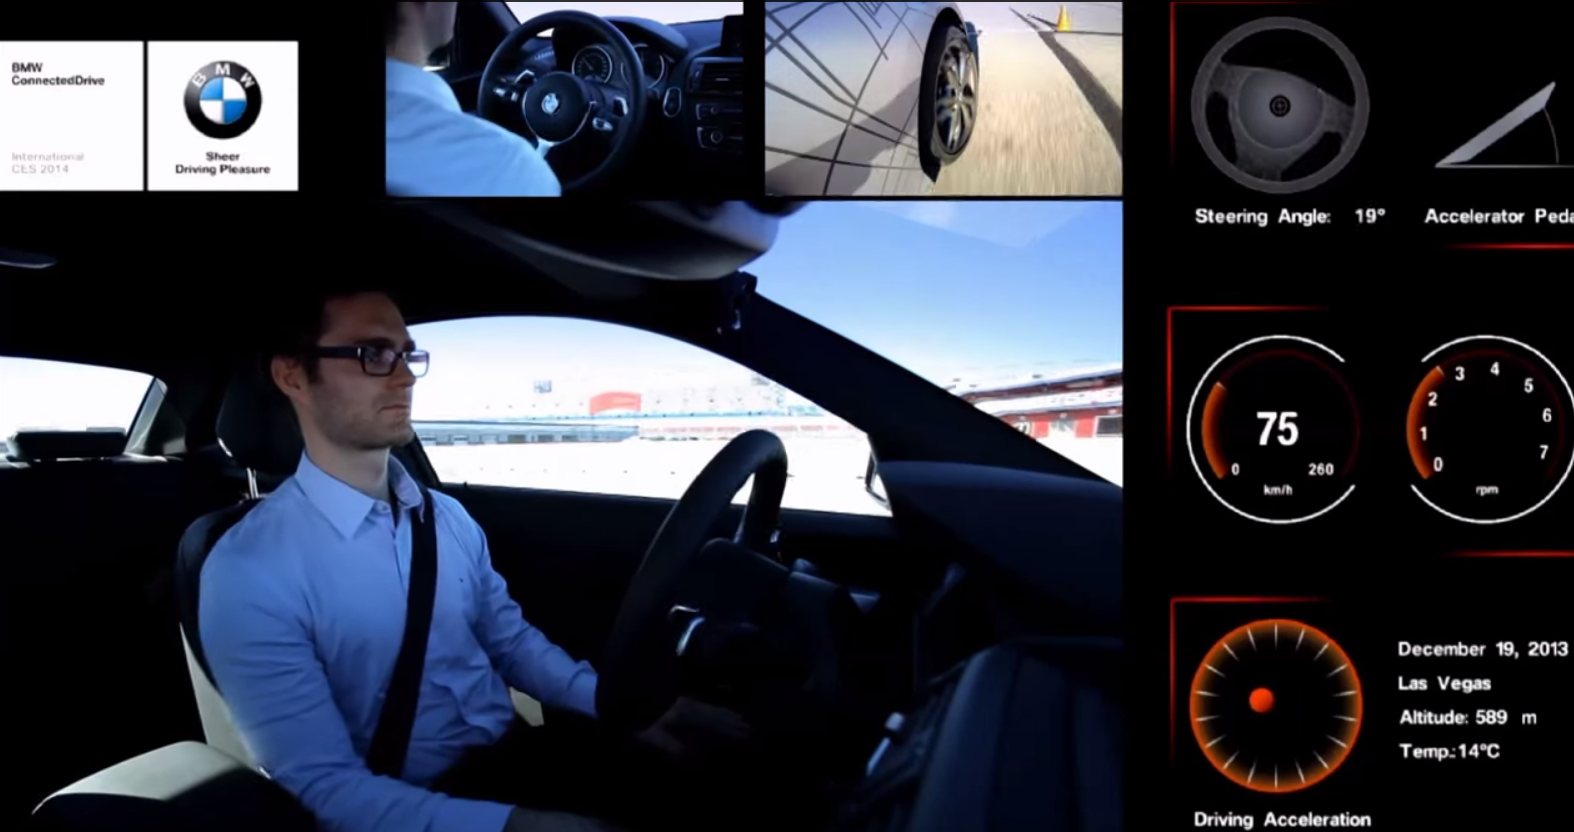
\includegraphics[scale=.7]{autonomous_car}
\end{figure}
\url{https://youtu.be/1FVglbJZ_tg}
\end{frame}

%------------------------------------------------

\begin{frame}
\frametitle{The Cubli: a cube that can jump, balance and 'walk'}
\begin{figure}
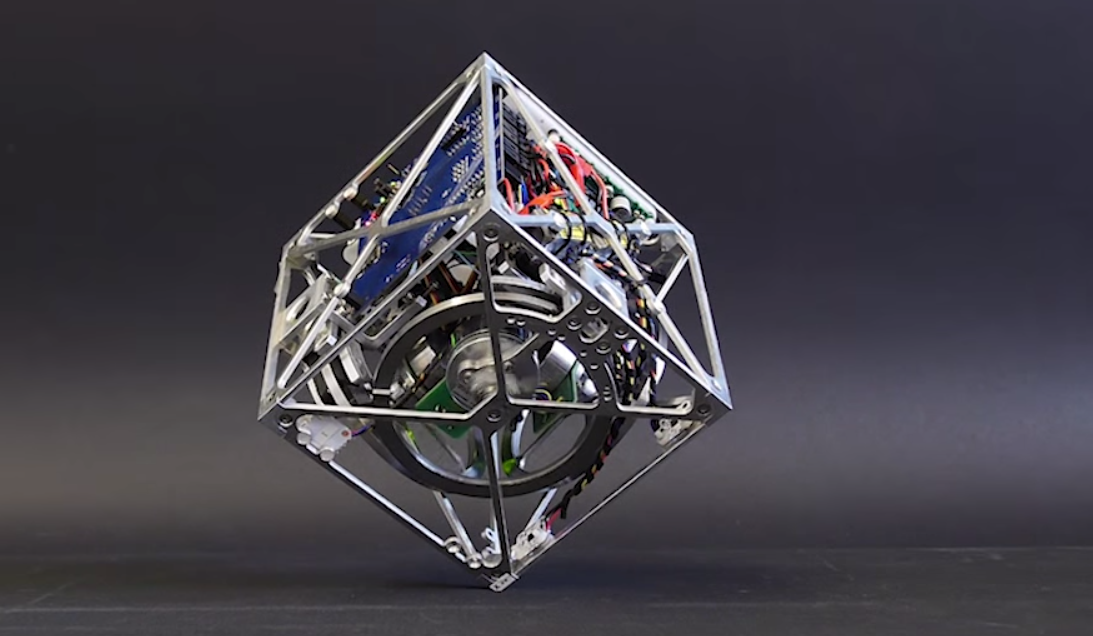
\includegraphics[scale=.7]{cubli}
\end{figure}
\url{https://youtu.be/n_6p-1J551Y}
\end{frame}

%------------------------------------------------

\begin{frame}
\frametitle{Magnetic manipulator Magman and Matlab}
\begin{figure}
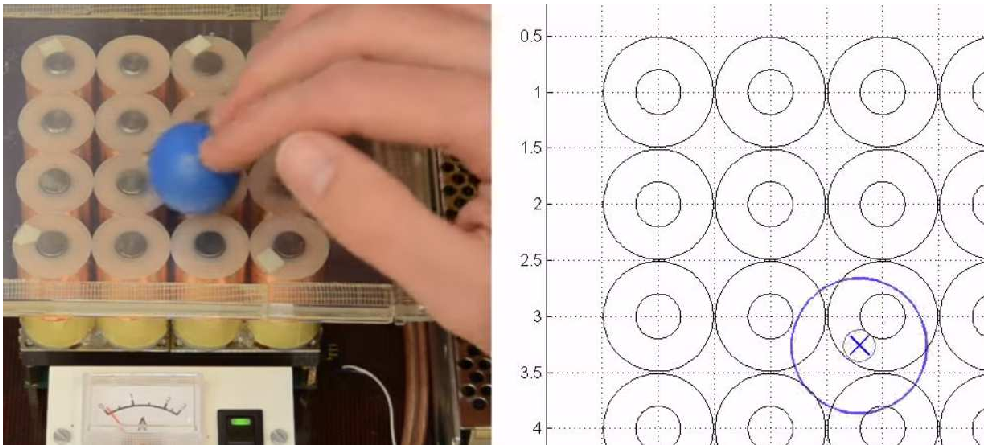
\includegraphics[scale=.7]{magnetic_manipulator}
\end{figure}
\url{https://youtu.be/AhS_2gU1qW0}
\end{frame}

%------------------------------------------------

\begin{frame}
\frametitle{Badminton robot}
\begin{figure}
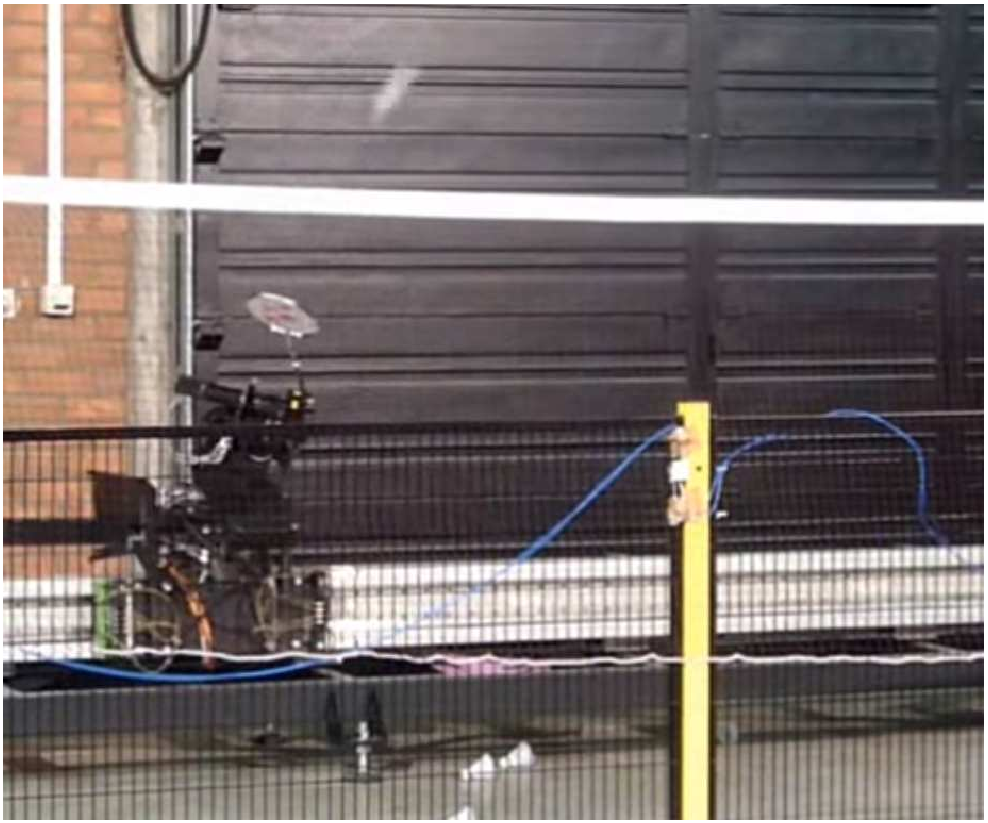
\includegraphics[scale=.5]{badminton_robot}
\end{figure}
\url{https://youtu.be/LSax71cn6A4}
\end{frame}

%------------------------------------------------

\begin{frame}
\frametitle{Raffaello D'Andrea: The astounding athletic power of quadcopters}
\begin{figure}
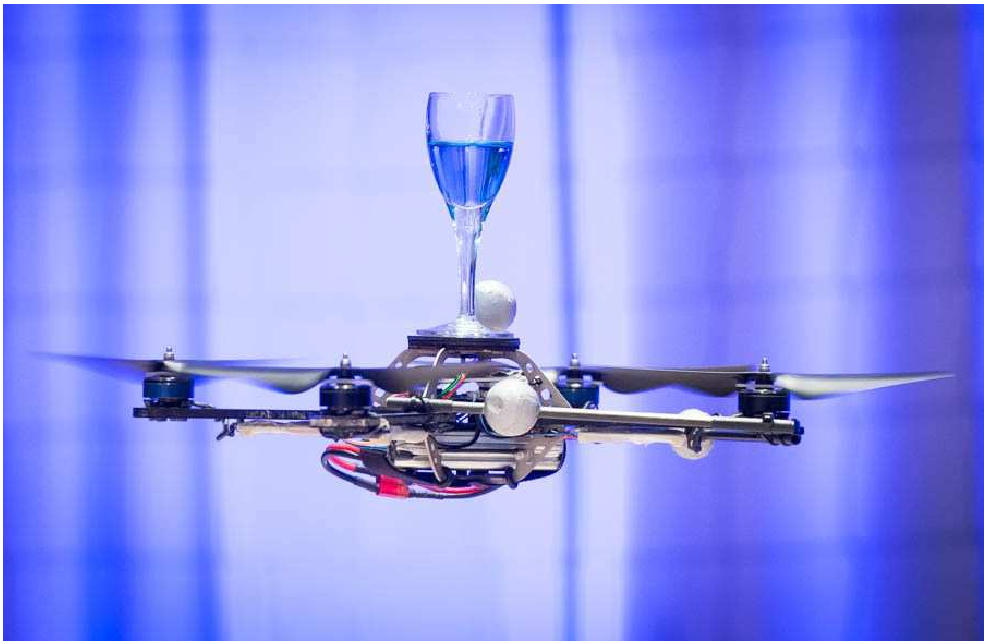
\includegraphics[scale=.6]{quadcopter}
\end{figure}
\url{https://www.youtube.com/watch?v=w2itwFJCgFQ}
\end{frame}

%------------------------------------------------
\end{document} 